This is pdfTeX, Version 3.14159265-2.6-1.40.20 (TeX Live 2019/Debian) (preloaded format=pdflatex)
 restricted \write18 enabled.
entering extended mode
(./main_uga.tex
LaTeX2e <2020-02-02> patch level 2
L3 programming layer <2020-02-14>
(/usr/share/texlive/texmf-dist/tex/latex/koma-script/scrreprt.cls
Document Class: scrreprt 2020/01/24 v3.29 KOMA-Script document class (report)
(/usr/share/texlive/texmf-dist/tex/latex/koma-script/scrkbase.sty
(/usr/share/texlive/texmf-dist/tex/latex/koma-script/scrbase.sty
(/usr/share/texlive/texmf-dist/tex/latex/graphics/keyval.sty)
(/usr/share/texlive/texmf-dist/tex/latex/koma-script/scrlfile.sty)))
(/usr/share/texlive/texmf-dist/tex/latex/koma-script/tocbasic.sty)
(/usr/share/texlive/texmf-dist/tex/latex/koma-script/scrsize11pt.clo)
(/usr/share/texlive/texmf-dist/tex/latex/koma-script/typearea.sty))
(./setup_thesis.tex (/usr/share/texlive/texmf-dist/tex/latex/base/inputenc.sty)
 (/usr/share/texlive/texmf-dist/tex/latex/base/fontenc.sty)
(/usr/share/texlive/texmf-dist/tex/latex/base/textcomp.sty)
(/usr/share/texlive/texmf-dist/tex/latex/todonotes/todonotes.sty
(/usr/share/texlive/texmf-dist/tex/latex/base/ifthen.sty)
(/usr/share/texlive/texmf-dist/tex/latex/xkeyval/xkeyval.sty
(/usr/share/texlive/texmf-dist/tex/generic/xkeyval/xkeyval.tex
(/usr/share/texlive/texmf-dist/tex/generic/xkeyval/xkvutils.tex)))
(/usr/share/texlive/texmf-dist/tex/latex/xcolor/xcolor.sty
(/usr/share/texlive/texmf-dist/tex/latex/graphics-cfg/color.cfg)
(/usr/share/texlive/texmf-dist/tex/latex/graphics-def/pdftex.def))
(/usr/share/texlive/texmf-dist/tex/latex/pgf/frontendlayer/tikz.sty
(/usr/share/texlive/texmf-dist/tex/latex/pgf/basiclayer/pgf.sty
(/usr/share/texlive/texmf-dist/tex/latex/pgf/utilities/pgfrcs.sty
(/usr/share/texlive/texmf-dist/tex/generic/pgf/utilities/pgfutil-common.tex
(/usr/share/texlive/texmf-dist/tex/generic/pgf/utilities/pgfutil-common-lists.t
ex)) (/usr/share/texlive/texmf-dist/tex/generic/pgf/utilities/pgfutil-latex.def
(/usr/share/texlive/texmf-dist/tex/latex/ms/everyshi.sty))
(/usr/share/texlive/texmf-dist/tex/generic/pgf/utilities/pgfrcs.code.tex
(/usr/share/texlive/texmf-dist/tex/generic/pgf/pgf.revision.tex)))
(/usr/share/texlive/texmf-dist/tex/latex/pgf/basiclayer/pgfcore.sty
(/usr/share/texlive/texmf-dist/tex/latex/graphics/graphicx.sty
(/usr/share/texlive/texmf-dist/tex/latex/graphics/graphics.sty
(/usr/share/texlive/texmf-dist/tex/latex/graphics/trig.sty)
(/usr/share/texlive/texmf-dist/tex/latex/graphics-cfg/graphics.cfg)))
(/usr/share/texlive/texmf-dist/tex/latex/pgf/systemlayer/pgfsys.sty
(/usr/share/texlive/texmf-dist/tex/generic/pgf/systemlayer/pgfsys.code.tex
(/usr/share/texlive/texmf-dist/tex/generic/pgf/utilities/pgfkeys.code.tex
(/usr/share/texlive/texmf-dist/tex/generic/pgf/utilities/pgfkeysfiltered.code.t
ex)) (/usr/share/texlive/texmf-dist/tex/generic/pgf/systemlayer/pgf.cfg)
(/usr/share/texlive/texmf-dist/tex/generic/pgf/systemlayer/pgfsys-pdftex.def
(/usr/share/texlive/texmf-dist/tex/generic/pgf/systemlayer/pgfsys-common-pdf.de
f)))
(/usr/share/texlive/texmf-dist/tex/generic/pgf/systemlayer/pgfsyssoftpath.code.
tex)
(/usr/share/texlive/texmf-dist/tex/generic/pgf/systemlayer/pgfsysprotocol.code.
tex))
(/usr/share/texlive/texmf-dist/tex/generic/pgf/basiclayer/pgfcore.code.tex
(/usr/share/texlive/texmf-dist/tex/generic/pgf/math/pgfmath.code.tex
(/usr/share/texlive/texmf-dist/tex/generic/pgf/math/pgfmathcalc.code.tex
(/usr/share/texlive/texmf-dist/tex/generic/pgf/math/pgfmathutil.code.tex)
(/usr/share/texlive/texmf-dist/tex/generic/pgf/math/pgfmathparser.code.tex)
(/usr/share/texlive/texmf-dist/tex/generic/pgf/math/pgfmathfunctions.code.tex
(/usr/share/texlive/texmf-dist/tex/generic/pgf/math/pgfmathfunctions.basic.code
.tex)
(/usr/share/texlive/texmf-dist/tex/generic/pgf/math/pgfmathfunctions.trigonomet
ric.code.tex)
(/usr/share/texlive/texmf-dist/tex/generic/pgf/math/pgfmathfunctions.random.cod
e.tex)
(/usr/share/texlive/texmf-dist/tex/generic/pgf/math/pgfmathfunctions.comparison
.code.tex)
(/usr/share/texlive/texmf-dist/tex/generic/pgf/math/pgfmathfunctions.base.code.
tex)
(/usr/share/texlive/texmf-dist/tex/generic/pgf/math/pgfmathfunctions.round.code
.tex)
(/usr/share/texlive/texmf-dist/tex/generic/pgf/math/pgfmathfunctions.misc.code.
tex)
(/usr/share/texlive/texmf-dist/tex/generic/pgf/math/pgfmathfunctions.integerari
thmetics.code.tex)))
(/usr/share/texlive/texmf-dist/tex/generic/pgf/math/pgfmathfloat.code.tex))
(/usr/share/texlive/texmf-dist/tex/generic/pgf/math/pgfint.code.tex)
(/usr/share/texlive/texmf-dist/tex/generic/pgf/basiclayer/pgfcorepoints.code.te
x)
(/usr/share/texlive/texmf-dist/tex/generic/pgf/basiclayer/pgfcorepathconstruct.
code.tex)
(/usr/share/texlive/texmf-dist/tex/generic/pgf/basiclayer/pgfcorepathusage.code
.tex)
(/usr/share/texlive/texmf-dist/tex/generic/pgf/basiclayer/pgfcorescopes.code.te
x)
(/usr/share/texlive/texmf-dist/tex/generic/pgf/basiclayer/pgfcoregraphicstate.c
ode.tex)
(/usr/share/texlive/texmf-dist/tex/generic/pgf/basiclayer/pgfcoretransformation
s.code.tex)
(/usr/share/texlive/texmf-dist/tex/generic/pgf/basiclayer/pgfcorequick.code.tex
)
(/usr/share/texlive/texmf-dist/tex/generic/pgf/basiclayer/pgfcoreobjects.code.t
ex)
(/usr/share/texlive/texmf-dist/tex/generic/pgf/basiclayer/pgfcorepathprocessing
.code.tex)
(/usr/share/texlive/texmf-dist/tex/generic/pgf/basiclayer/pgfcorearrows.code.te
x)
(/usr/share/texlive/texmf-dist/tex/generic/pgf/basiclayer/pgfcoreshade.code.tex
)
(/usr/share/texlive/texmf-dist/tex/generic/pgf/basiclayer/pgfcoreimage.code.tex

(/usr/share/texlive/texmf-dist/tex/generic/pgf/basiclayer/pgfcoreexternal.code.
tex))
(/usr/share/texlive/texmf-dist/tex/generic/pgf/basiclayer/pgfcorelayers.code.te
x)
(/usr/share/texlive/texmf-dist/tex/generic/pgf/basiclayer/pgfcoretransparency.c
ode.tex)
(/usr/share/texlive/texmf-dist/tex/generic/pgf/basiclayer/pgfcorepatterns.code.
tex)
(/usr/share/texlive/texmf-dist/tex/generic/pgf/basiclayer/pgfcorerdf.code.tex))
)
(/usr/share/texlive/texmf-dist/tex/generic/pgf/modules/pgfmoduleshapes.code.tex
) (/usr/share/texlive/texmf-dist/tex/generic/pgf/modules/pgfmoduleplot.code.tex
)
(/usr/share/texlive/texmf-dist/tex/latex/pgf/compatibility/pgfcomp-version-0-65
.sty)
(/usr/share/texlive/texmf-dist/tex/latex/pgf/compatibility/pgfcomp-version-1-18
.sty)) (/usr/share/texlive/texmf-dist/tex/latex/pgf/utilities/pgffor.sty
(/usr/share/texlive/texmf-dist/tex/latex/pgf/utilities/pgfkeys.sty
(/usr/share/texlive/texmf-dist/tex/generic/pgf/utilities/pgfkeys.code.tex))
(/usr/share/texlive/texmf-dist/tex/latex/pgf/math/pgfmath.sty
(/usr/share/texlive/texmf-dist/tex/generic/pgf/math/pgfmath.code.tex))
(/usr/share/texlive/texmf-dist/tex/generic/pgf/utilities/pgffor.code.tex
(/usr/share/texlive/texmf-dist/tex/generic/pgf/math/pgfmath.code.tex)))
(/usr/share/texlive/texmf-dist/tex/generic/pgf/frontendlayer/tikz/tikz.code.tex

(/usr/share/texlive/texmf-dist/tex/generic/pgf/libraries/pgflibraryplothandlers
.code.tex)
(/usr/share/texlive/texmf-dist/tex/generic/pgf/modules/pgfmodulematrix.code.tex
)
(/usr/share/texlive/texmf-dist/tex/generic/pgf/frontendlayer/tikz/libraries/tik
zlibrarytopaths.code.tex)))
(/usr/share/texlive/texmf-dist/tex/generic/pgf/frontendlayer/tikz/libraries/tik
zlibrarypositioning.code.tex)
(/usr/share/texlive/texmf-dist/tex/generic/pgf/frontendlayer/tikz/libraries/tik
zlibraryshadows.code.tex
(/usr/share/texlive/texmf-dist/tex/generic/pgf/frontendlayer/tikz/libraries/tik
zlibraryfadings.code.tex
(/usr/share/texlive/texmf-dist/tex/generic/pgf/libraries/pgflibraryfadings.code
.tex))) (/usr/share/texlive/texmf-dist/tex/latex/tools/calc.sty))
(/usr/share/texlive/texmf-dist/tex/generic/pgf/frontendlayer/tikz/libraries/tik
zlibraryarrows.code.tex
(/usr/share/texlive/texmf-dist/tex/generic/pgf/libraries/pgflibraryarrows.code.
tex))
(/usr/share/texlive/texmf-dist/tex/generic/pgf/frontendlayer/tikz/libraries/tik
zlibraryshapes.code.tex
(/usr/share/texlive/texmf-dist/tex/generic/pgf/frontendlayer/tikz/libraries/tik
zlibraryshapes.geometric.code.tex
(/usr/share/texlive/texmf-dist/tex/generic/pgf/libraries/shapes/pgflibraryshape
s.geometric.code.tex))
(/usr/share/texlive/texmf-dist/tex/generic/pgf/frontendlayer/tikz/libraries/tik
zlibraryshapes.misc.code.tex
(/usr/share/texlive/texmf-dist/tex/generic/pgf/libraries/shapes/pgflibraryshape
s.misc.code.tex))
(/usr/share/texlive/texmf-dist/tex/generic/pgf/frontendlayer/tikz/libraries/tik
zlibraryshapes.symbols.code.tex
(/usr/share/texlive/texmf-dist/tex/generic/pgf/libraries/shapes/pgflibraryshape
s.symbols.code.tex))
(/usr/share/texlive/texmf-dist/tex/generic/pgf/frontendlayer/tikz/libraries/tik
zlibraryshapes.arrows.code.tex
(/usr/share/texlive/texmf-dist/tex/generic/pgf/libraries/shapes/pgflibraryshape
s.arrows.code.tex))
(/usr/share/texlive/texmf-dist/tex/generic/pgf/frontendlayer/tikz/libraries/tik
zlibraryshapes.callouts.code.tex
(/usr/share/texlive/texmf-dist/tex/generic/pgf/libraries/shapes/pgflibraryshape
s.callouts.code.tex))
(/usr/share/texlive/texmf-dist/tex/generic/pgf/frontendlayer/tikz/libraries/tik
zlibraryshapes.multipart.code.tex
(/usr/share/texlive/texmf-dist/tex/generic/pgf/libraries/shapes/pgflibraryshape
s.multipart.code.tex)))
(/usr/share/texlive/texmf-dist/tex/latex/psnfss/pifont.sty
(/usr/share/texlive/texmf-dist/tex/latex/psnfss/upzd.fd)
(/usr/share/texlive/texmf-dist/tex/latex/psnfss/upsy.fd))
(/usr/share/texlive/texmf-dist/tex/latex/hyperref/hyperref.sty
(/usr/share/texlive/texmf-dist/tex/generic/ltxcmds/ltxcmds.sty)
(/usr/share/texlive/texmf-dist/tex/generic/iftex/iftex.sty)
(/usr/share/texlive/texmf-dist/tex/latex/pdftexcmds/pdftexcmds.sty
(/usr/share/texlive/texmf-dist/tex/generic/infwarerr/infwarerr.sty))
(/usr/share/texlive/texmf-dist/tex/generic/kvsetkeys/kvsetkeys.sty)
(/usr/share/texlive/texmf-dist/tex/generic/kvdefinekeys/kvdefinekeys.sty)
(/usr/share/texlive/texmf-dist/tex/generic/pdfescape/pdfescape.sty)
(/usr/share/texlive/texmf-dist/tex/latex/hycolor/hycolor.sty)
(/usr/share/texlive/texmf-dist/tex/latex/letltxmacro/letltxmacro.sty)
(/usr/share/texlive/texmf-dist/tex/latex/auxhook/auxhook.sty)
(/usr/share/texlive/texmf-dist/tex/latex/kvoptions/kvoptions.sty)
(/usr/share/texlive/texmf-dist/tex/latex/hyperref/pd1enc.def)
(/usr/share/texlive/texmf-dist/tex/generic/intcalc/intcalc.sty)
(/usr/share/texlive/texmf-dist/tex/generic/etexcmds/etexcmds.sty)
(/usr/share/texlive/texmf-dist/tex/latex/url/url.sty)
(/usr/share/texlive/texmf-dist/tex/generic/bitset/bitset.sty
(/usr/share/texlive/texmf-dist/tex/generic/bigintcalc/bigintcalc.sty))
(/usr/share/texlive/texmf-dist/tex/generic/atbegshi/atbegshi.sty))
(/usr/share/texlive/texmf-dist/tex/latex/hyperref/hpdftex.def
(/usr/share/texlive/texmf-dist/tex/latex/atveryend/atveryend.sty)
(/usr/share/texlive/texmf-dist/tex/latex/rerunfilecheck/rerunfilecheck.sty
(/usr/share/texlive/texmf-dist/tex/generic/uniquecounter/uniquecounter.sty)))
(/usr/share/texlive/texmf-dist/tex/latex/calculator/calculus.sty
(/usr/share/texlive/texmf-dist/tex/latex/calculator/calculator.sty))
(/usr/share/texlive/texmf-dist/tex/latex/listings/listings.sty
(/usr/share/texlive/texmf-dist/tex/latex/listings/lstmisc.sty)
(/usr/share/texlive/texmf-dist/tex/latex/listings/listings.cfg))
(/usr/share/texlive/texmf-dist/tex/latex/xurl/xurl.sty)
(/usr/share/texlive/texmf-dist/tex/latex/graphics/epsfig.sty)
(/usr/share/texlive/texmf-dist/tex/latex/tools/multicol.sty)
(/usr/share/texlive/texmf-dist/tex/latex/pslatex/pslatex.sty)
(/usr/share/texlive/texmf-dist/tex/latex/siunitx/siunitx.sty
(/usr/share/texlive/texmf-dist/tex/latex/l3kernel/expl3.sty
(/usr/share/texlive/texmf-dist/tex/latex/l3backend/l3backend-pdfmode.def))
(/usr/share/texlive/texmf-dist/tex/latex/l3packages/xparse/xparse.sty)
(/usr/share/texlive/texmf-dist/tex/latex/amsmath/amstext.sty
(/usr/share/texlive/texmf-dist/tex/latex/amsmath/amsgen.sty))
(/usr/share/texlive/texmf-dist/tex/latex/tools/array.sty)
(/usr/share/texlive/texmf-dist/tex/latex/l3packages/l3keys2e/l3keys2e.sty)
(/usr/share/texlive/texmf-dist/tex/latex/translator/translator.sty))
(/usr/share/texlive/texmf-dist/tex/latex/chemformula/chemformula.sty
(/usr/share/texlive/texmf-dist/tex/latex/amsmath/amsmath.sty
For additional information on amsmath, use the `?' option.
(/usr/share/texlive/texmf-dist/tex/latex/amsmath/amsbsy.sty)
(/usr/share/texlive/texmf-dist/tex/latex/amsmath/amsopn.sty))
(/usr/share/texlive/texmf-dist/tex/latex/l3packages/xfrac/xfrac.sty
(/usr/share/texlive/texmf-dist/tex/latex/l3packages/xtemplate/xtemplate.sty))
(/usr/share/texlive/texmf-dist/tex/latex/units/nicefrac.sty)
(/usr/share/texlive/texmf-dist/tex/generic/pgf/libraries/pgflibraryarrows.meta.
code.tex)) (/usr/share/texlive/texmf-dist/tex/latex/comment/comment.sty
Excluding comment 'comment') (./sty/uga.sty

LaTeX Warning: You have requested package `sty/uga',
               but the package provides `uga'.

(/usr/share/texlive/texmf-dist/tex/latex/svg/svg.sty
(/usr/share/texlive/texmf-dist/tex/latex/tools/shellesc.sty)
(/usr/share/texlive/texmf-dist/tex/latex/trimspaces/trimspaces.sty))
(/usr/share/texlive/texmf-dist/tex/latex/transparent/transparent.sty))
(/usr/share/texlive/texmf-dist/tex/latex/setspace/setspace.sty)
(/usr/share/texlive/texmf-dist/tex/latex/standalone/standalone.sty
(/usr/share/texlive/texmf-dist/tex/latex/currfile/currfile.sty
(/usr/share/texlive/texmf-dist/tex/latex/filehook/filehook.sty
(/usr/share/texlive/texmf-dist/tex/latex/filehook/filehook-scrlfile.sty)))
(/usr/share/texlive/texmf-dist/tex/latex/gincltex/gincltex.sty
(/usr/share/texlive/texmf-dist/tex/latex/svn-prov/svn-prov.sty)
(/usr/share/texlive/texmf-dist/tex/latex/adjustbox/adjustbox.sty
(/usr/share/texlive/texmf-dist/tex/latex/adjustbox/adjcalc.sty)
(/usr/share/texlive/texmf-dist/tex/latex/adjustbox/trimclip.sty
(/usr/share/texlive/texmf-dist/tex/latex/collectbox/collectbox.sty)
(/usr/share/texlive/texmf-dist/tex/latex/adjustbox/tc-pdftex.def))
(/usr/share/texlive/texmf-dist/tex/latex/ifoddpage/ifoddpage.sty)
(/usr/share/texlive/texmf-dist/tex/latex/varwidth/varwidth.sty)))
(/usr/share/texlive/texmf-dist/tex/latex/filemod/filemod-expmin.sty))
(/usr/share/texlive/texmf-dist/tex/latex/caption/caption.sty
(/usr/share/texlive/texmf-dist/tex/latex/caption/caption3.sty))
(/usr/share/texlive/texmf-dist/tex/generic/pgf/frontendlayer/tikz/libraries/tik
zlibrarybabel.code.tex)
(/usr/share/texlive/texmf-dist/tex/generic/pgf/frontendlayer/tikz/libraries/tik
zlibrarycalc.code.tex)
(/usr/share/texlive/texmf-dist/tex/generic/pgf/frontendlayer/tikz/libraries/tik
zlibraryfit.code.tex)
(/usr/share/texlive/texmf-dist/tex/generic/pgf/frontendlayer/tikz/libraries/gra
phs/tikzlibrarygraphs.code.tex)
(/usr/share/texlive/texmf-dist/tex/generic/pgf/frontendlayer/tikz/libraries/gra
phs/tikzlibrarygraphs.standard.code.tex)
(/usr/share/texlive/texmf-dist/tex/generic/pgf/frontendlayer/tikz/libraries/tik
zlibrarypatterns.code.tex
(/usr/share/texlive/texmf-dist/tex/generic/pgf/libraries/pgflibrarypatterns.cod
e.tex)) (/usr/share/texlive/texmf-dist/tex/latex/algorithms/algorithm.sty
(/usr/share/texlive/texmf-dist/tex/latex/float/float.sty))
(/usr/share/texlive/texmf-dist/tex/latex/algorithmicx/algpseudocode.sty
(/usr/share/texlive/texmf-dist/tex/latex/algorithmicx/algorithmicx.sty
Document Style algorithmicx 1.2 - a greatly improved `algorithmic' style
)
Document Style - pseudocode environments for use with the `algorithmicx' style
) (/usr/share/texlive/texmf-dist/tex/latex/amsfonts/amssymb.sty
(/usr/share/texlive/texmf-dist/tex/latex/amsfonts/amsfonts.sty))
(/usr/share/texlive/texmf-dist/tex/latex/amscls/amsthm.sty)
(/usr/share/texlive/texmf-dist/tex/latex/xpatch/xpatch.sty
(/usr/share/texlive/texmf-dist/tex/latex/etoolbox/etoolbox.sty))
(/usr/share/texlive/texmf-dist/tex/latex/booktabs/booktabs.sty)
(/usr/share/texlive/texmf-dist/tex/latex/multirow/multirow.sty)
(/usr/share/texlive/texmf-dist/tex/generic/babel/babel.sty
(/usr/share/texlive/texmf-dist/tex/generic/babel/switch.def)
(/usr/share/texlive/texmf-dist/tex/generic/babel-french/french.ldf
(/usr/share/texlive/texmf-dist/tex/generic/babel/babel.def
(/usr/share/texlive/texmf-dist/tex/generic/babel/txtbabel.def)))
(/usr/share/texlive/texmf-dist/tex/generic/babel-english/english.ldf))
(/usr/share/texlive/texmf-dist/tex/latex/carlisle/scalefnt.sty)
(/usr/share/texlive/texmf-dist/tex/latex/isodate/isodate.sty
(/usr/share/texlive/texmf-dist/tex/latex/substr/substr.sty)
(/usr/share/texlive/texmf-dist/tex/latex/isodate/french.idf
Define commands for French date format
) (/usr/share/texlive/texmf-dist/tex/latex/isodate/english.idf
Define commands for English date format
)) (/usr/share/texlive/texmf-dist/tex/latex/cleanthesis/cleanthesis.sty
(/usr/share/texlive/texmf-dist/tex/latex/base/fontenc.sty)
(/usr/share/texmf/tex/latex/lm/lmodern.sty)
(/usr/share/texlive/texmf-dist/tex/latex/psnfss/charter.sty)
(/usr/share/texlive/texmf-dist/tex/latex/microtype/microtype.sty
(/usr/share/texlive/texmf-dist/tex/latex/microtype/microtype-pdftex.def)
(/usr/share/texlive/texmf-dist/tex/latex/microtype/microtype.cfg))
(/usr/share/texlive/texmf-dist/tex/latex/tools/tabularx.sty)
(/usr/share/texlive/texmf-dist/tex/latex/enumitem/enumitem.sty)
(/usr/share/texlive/texmf-dist/tex/latex/blindtext/blindtext.sty
(/usr/share/texlive/texmf-dist/tex/latex/tools/xspace.sty))
(/usr/share/texlive/texmf-dist/tex/latex/koma-script/scrlayer-scrpage.sty
(/usr/share/texlive/texmf-dist/tex/latex/koma-script/scrlayer.sty))
1: section
1: chapter
1: chapter
1: section
(/usr/share/texlive/texmf-dist/tex/latex/psnfss/t1bch.fd)
(/usr/share/texlive/texmf-dist/tex/latex/csquotes/csquotes.sty
(/usr/share/texlive/texmf-dist/tex/latex/csquotes/csquotes.def)
(/usr/share/texlive/texmf-dist/tex/latex/csquotes/csquotes.cfg))
(/usr/share/texlive/texmf-dist/tex/latex/biblatex/biblatex.sty
(/usr/share/texlive/texmf-dist/tex/latex/logreq/logreq.sty
(/usr/share/texlive/texmf-dist/tex/latex/logreq/logreq.def))
(/usr/share/texlive/texmf-dist/tex/latex/biblatex/blx-dm.def)
(/usr/share/texlive/texmf-dist/tex/latex/biblatex/blx-compat.def)
(/usr/share/texlive/texmf-dist/tex/latex/biblatex/biblatex.def)
(/usr/share/texlive/texmf-dist/tex/latex/biblatex/blx-natbib.def)
(/usr/share/texlive/texmf-dist/tex/latex/biblatex/bbx/numeric.bbx
(/usr/share/texlive/texmf-dist/tex/latex/biblatex/bbx/standard.bbx))
(/usr/share/texlive/texmf-dist/tex/latex/biblatex/cbx/numeric.cbx)
(/usr/share/texlive/texmf-dist/tex/latex/biblatex/biblatex.cfg))
1: section
1: chapter
1: chapter
1: section

Class scrreprt Warning: Usage of package `tocloft' together
(scrreprt)              with a KOMA-Script class is not recommended.
(scrreprt)              I'd suggest to use options like `listof=entryprefix',
(scrreprt)              commands like `\listoflofentryname' or
(scrreprt)              `\listoflotentryname', and `\DeclareTOCStyleEntry' or
(scrreprt)              `\RedeclareSectionCommand' instead of this package,
(scrreprt)              because it breaks several KOMA-Script features of
(scrreprt)              the list of figures, list of tables and table of
(scrreprt)              contents, i.e., options like `listof=numbered',
(scrreprt)              `listof=flat or `toc=flat', commands like
(scrreprt)              `\BeforeTOCHead{...}' and `\AfterTOCHead{...}',
(scrreprt)              `\BeforeStartingTOC{...}' and \AfterStartingTOC{...}',
(scrreprt)              all features of `\DeclareTOCStyleEntry',
(scrreprt)              and the ToC entry features of `\DeclareSecionCommand'
(scrreprt)              and `\RedeclareSectionCommand' of levels
(scrreprt)              `part', `section', `subsection',
(scrreprt)              `subsubsection', `paragraph' and `subparagraph'.
(scrreprt)              Nevertheless, using requested
(scrreprt)              package `tocloft' on input line 693.

(/usr/share/texlive/texmf-dist/tex/latex/tocloft/tocloft.sty))
(/usr/share/texlive/texmf-dist/tex/latex/hyperref/puenc.def)) (./main_uga.aux

LaTeX Warning: Label `fig:pv_ghi' multiply defined.


LaTeX Warning: Label `tab:carbonfootprint' multiply defined.

) (/usr/share/texlive/texmf-dist/tex/latex/psnfss/omspzccm.fd)
(/usr/share/texlive/texmf-dist/tex/context/base/mkii/supp-pdf.mkii
[Loading MPS to PDF converter (version 2006.09.02).]
) (/usr/share/texlive/texmf-dist/tex/latex/epstopdf-pkg/epstopdf-base.sty
(/usr/share/texlive/texmf-dist/tex/latex/latexconfig/epstopdf-sys.cfg))
ABD: EveryShipout initializing macros
(/usr/share/texlive/texmf-dist/tex/latex/hyperref/nameref.sty
(/usr/share/texlive/texmf-dist/tex/latex/refcount/refcount.sty)
(/usr/share/texlive/texmf-dist/tex/generic/gettitlestring/gettitlestring.sty))
(./main_uga.out) (./main_uga.out)
(/usr/share/texlive/texmf-dist/tex/latex/bookmark/bookmark.sty
(/usr/share/texlive/texmf-dist/tex/latex/bookmark/bkm-pdftex.def))
(/usr/share/texlive/texmf-dist/tex/latex/translator/translator-basic-dictionary
-English.dict)
(/usr/share/texlive/texmf-dist/tex/latex/siunitx/siunitx-abbreviations.cfg)

Package french.ldf Warning: Please load the "listings" package
(french.ldf)                AFTER babel/french; reported on input line 72.

isodate: babel.sty has been loaded
(/usr/share/texlive/texmf-dist/tex/latex/microtype/mt-bch.cfg)
(/usr/share/texlive/texmf-dist/tex/latex/biblatex/lbx/english.lbx)
(/usr/share/texlive/texmf-dist/tex/latex/biblatex/lbx/french.lbx)
(./main_uga.bbl

Package biblatex Warning: Biber reported the following issues
(biblatex)                with 'pv_lcoe_calc':
(biblatex)                - Entry 'pv_lcoe_calc' (references.bib): Invalid form
at '2021-8' of date field 'date' - ignoring.

) (/usr/share/texmf/tex/latex/lm/ot1lmr.fd)
(/usr/share/texlive/texmf-dist/tex/latex/microtype/mt-cmr.cfg)
(/usr/share/texmf/tex/latex/lm/omllmm.fd)
(/usr/share/texmf/tex/latex/lm/omslmsy.fd)
(/usr/share/texmf/tex/latex/lm/omxlmex.fd)
(/usr/share/texlive/texmf-dist/tex/latex/microtype/mt-ptm.cfg)
(/usr/share/texlive/texmf-dist/tex/latex/amsfonts/umsa.fd)
(/usr/share/texlive/texmf-dist/tex/latex/microtype/mt-msa.cfg)
(/usr/share/texlive/texmf-dist/tex/latex/amsfonts/umsb.fd)
(/usr/share/texlive/texmf-dist/tex/latex/microtype/mt-msb.cfg)
(/usr/share/texmf/tex/latex/lm/ot1lmss.fd)
(/usr/share/texmf/tex/latex/lm/ot1lmtt.fd) (./titlepage.tex [1{/var/lib/texmf/f
onts/map/pdftex/updmap/pdftex.map}]
! Argument of \Depot has an extra }.
<inserted text> 
                \par 
l.52 \MakeUGthesePDG
                      % actually generate the title page
? 
! Emergency stop.
<inserted text> 
                \par 
l.52 \MakeUGthesePDG
                      % actually generate the title page
!  ==> Fatal error occurred, no output PDF file produced!
Transcript written on main_uga.log.
\section{Introduction}

In the previous chapter, we presented an initial modeling to reduce the carbon emissions of operating a cloud federation for the short term (one year) by sizing its renewable infrastructure, that is, defining the area of solar panels and capacity of the batteries for each data center.  Given that the cloud federation will operate for the long term, the decision-maker needs to be sure of the investments that will be made to avoid wasting money and as well generating more environmental impact with a bad strategy. Furthermore, a planing process is subject to many uncertainties that if not taken into account will decrease the validity and credibility of the solution.

The reduction on the carbon emissions by using solar panels is limited by the fact that they only generates power when the sun is shinning, therefore they need to supply the operations of the cloud during the day and charge the batteries for night operations. In this chapter we will evaluate if using wind turbines could further reduce the carbon emissions of the cloud operation, and the sizing of both the PV panels and batteries --- considering that the wind may also be available at night.

One must also take into account that once built the renewable infrastructure cannot be reduced --- this would imply on destroying/discarding PV panels, batteries, and wind turbines therefore another strategy is necessary to deal with the over-sizing that might be caused by the intermittency of renewables sources. Thankfully, there is another part that can be managed to reduce the impact of bad-sizing: scheduling of the workload. In cloud platform, a significant part of the workload are tasks that does not have a high prioriry and whose execution can be delayed over time, the so-called batch tasks. We will show an analysis of the vialbiliy of if delaying $\alpha$ \% of the tasks up  to $\beta$ time slots (each time slot has 1 hour of duration) to reduce the carbon footprint.

Another important aspect to consider is that the demand for cloud computing resources grows year by year --- to deal with the increasing number of users and request of applications, and each year new servers generations are launched that have hardware more computational powerfull and that may be more energy efficient. As show by \citet{masanet2020recalibrating}, from 2010 to 2018 the DC workload increased 6 times, however the increase in energy consumption was only 6\% thanks to efficiency improvements in both hardware and software.  On the other hand, manufacturing these serves also emmits carbon and this cannot be neglected. Furthermore, given the increasing integration of renewable infrastructures in the cloud data centers, most of carbon emissions are shifting from the power consumption of the DC operation to the manufacturing of IT equipment \cite{gupta2021_chasingcarbon}.

This chapter will present an extension of the model focusing on the long-term operation of the cloud DCs and the uncertainties that this sizing process is subject to. More specifically, the chapter presents the following contributions:

\begin{itemize}
 
\item we extend the modeling to account for all the life cycle emissions of the renewable infrastructure --- from manufacturing to discarding/recycling

\item we present an evaluation of how much the carbon footprint could be reduced if wind turbines are also included in the renewable infrastructure 

\item we will show an evaluation regarding the sensitivity of the LP to the inputs: i) uncertainties caused by the intermittency of solar irradiation, and what needs to be considered in the modeling to avoid over or under-sizing of the PV panels; ii) some locations have data sources with grid carbon footprint at time intervals of one hour, and we will show an analysis if this fine-grain value would affect the renewable infrastructure sizing
  
\item we will how much we can reduce the carbon footprint using the flexibility of the schedulling --- delaying batch tasks 
 
\item we will show an analysis of how expensive (in dolars) is to reduce the cloud federation footprint and the gains in both monetary and emissions savings --- the monetary costs is other variable of high importance for the cloud operators, since the business will only survive if it generates profit

\item we will present an analysis of when is viable to add new servers (that may replace servers from older generations) in terms of carbon footprint

 
\end{itemize}

The remaining of the chapter is organized as follows. Considering that we are extending the model of the previous Chapter to evaluate different scenarios, each scenario will have its own Section --- Sections X, Y, Z, and in each section the reader will find the necessary modifications in the modeling, the experiments performed and the results of the experiments. After presenting the evaluated scenarios, we will show the discussion at Section. Finally, Section Z concludes the chapter.

\section{Life-cycle of the renewable infrastructure}

On the previous chapter, we made the modeling considering only the environmental impact of manufacturing the solar panels and the lithium-ion batteries. This decision was made because it was the avaiable data that we found at the time of studying the problem. However, the environmental impact also is present in the other phases of the life time of these devices --- as operation, discarding and recycling.

\subsection{Updates in the model}

Given that some sources provide the emissions for all the life cycle in terms of energy produced (or delivered in the case of the batteries) in $g\,\ch{CO2}-eq.Wh^{-1}$ we need to update the modeling to support these values. Equation~\eqref{eq:fppv_lca} models the new footprint for the PV panels, and the main difference is the $pvCO2LC$ input that represents the life-cicle emissions.

\begin{equation} \label{eq:fppv_lca}
   FPpv^d_k =  pvCO2LC \times Pre_k^d \times \Delta t
\end{equation}


For the batteries, the initial modeling considered the emissions of manufacturing related to its capacity. Now to account for all the life-cicle, the emissions relate to the energy delivered (discharged) by the batteries. Equation~\eqref{eq:fbat_lca} models the new footprint for batteries, where $batCO2LC$ represents the life-cicle emissions. 

\begin{equation} \label{eq:fbat_lca}
   FPbat^d_k =  Pdch^d_k \times batCO2LC
 \end{equation}
 
Considering that now the only information used for computing the emissions from the batteries is the power discharged, we need to add a restriction for the batteries being used only for night computations, otherwise the solver will compute a solution where the batteries will be oversized to store all the excess of renewable energy during summer to supply during winter, resulting in GWh of capacity --- which is a problem considering the other environmental impact of batteries as their recycle rates needs yet to improve. Equation~\eqref{eq:b_initial_level}  models this resctriction, where $SUNRISE^d$ is the set with all the instants of times where the sun starts shining throghout the year in each location considering its time zone.

\begin{equation} \label{eq:b_initial_level}
  \forall t \in SUNRISE^d :  B^d_t =  0.2 \times Bat^d
\end{equation}

\subsection{Experiments}
\label{sec:ex_lca_pv}

\subsubsection{Settings} 

The cloud infrastructure, the workload, grid emissions, and the execution environment are the same as in Section  \ref{sec:settings_ccgrid}. For the photovoltaic power production, we will use the average of the irradiation from the years 1980 to 2019, and Figure \ref{fig:pv_ghi_avg} illustrates the values for the different DCs locations. This modification was to consider the variations between the years, as using a single year is not enough: it may be the case of a year with lowest or highest solar irradiation. More details for choosing the average irradiation value will be given in the next section.

\begin{figure}[!htbp]  
  \centering
   {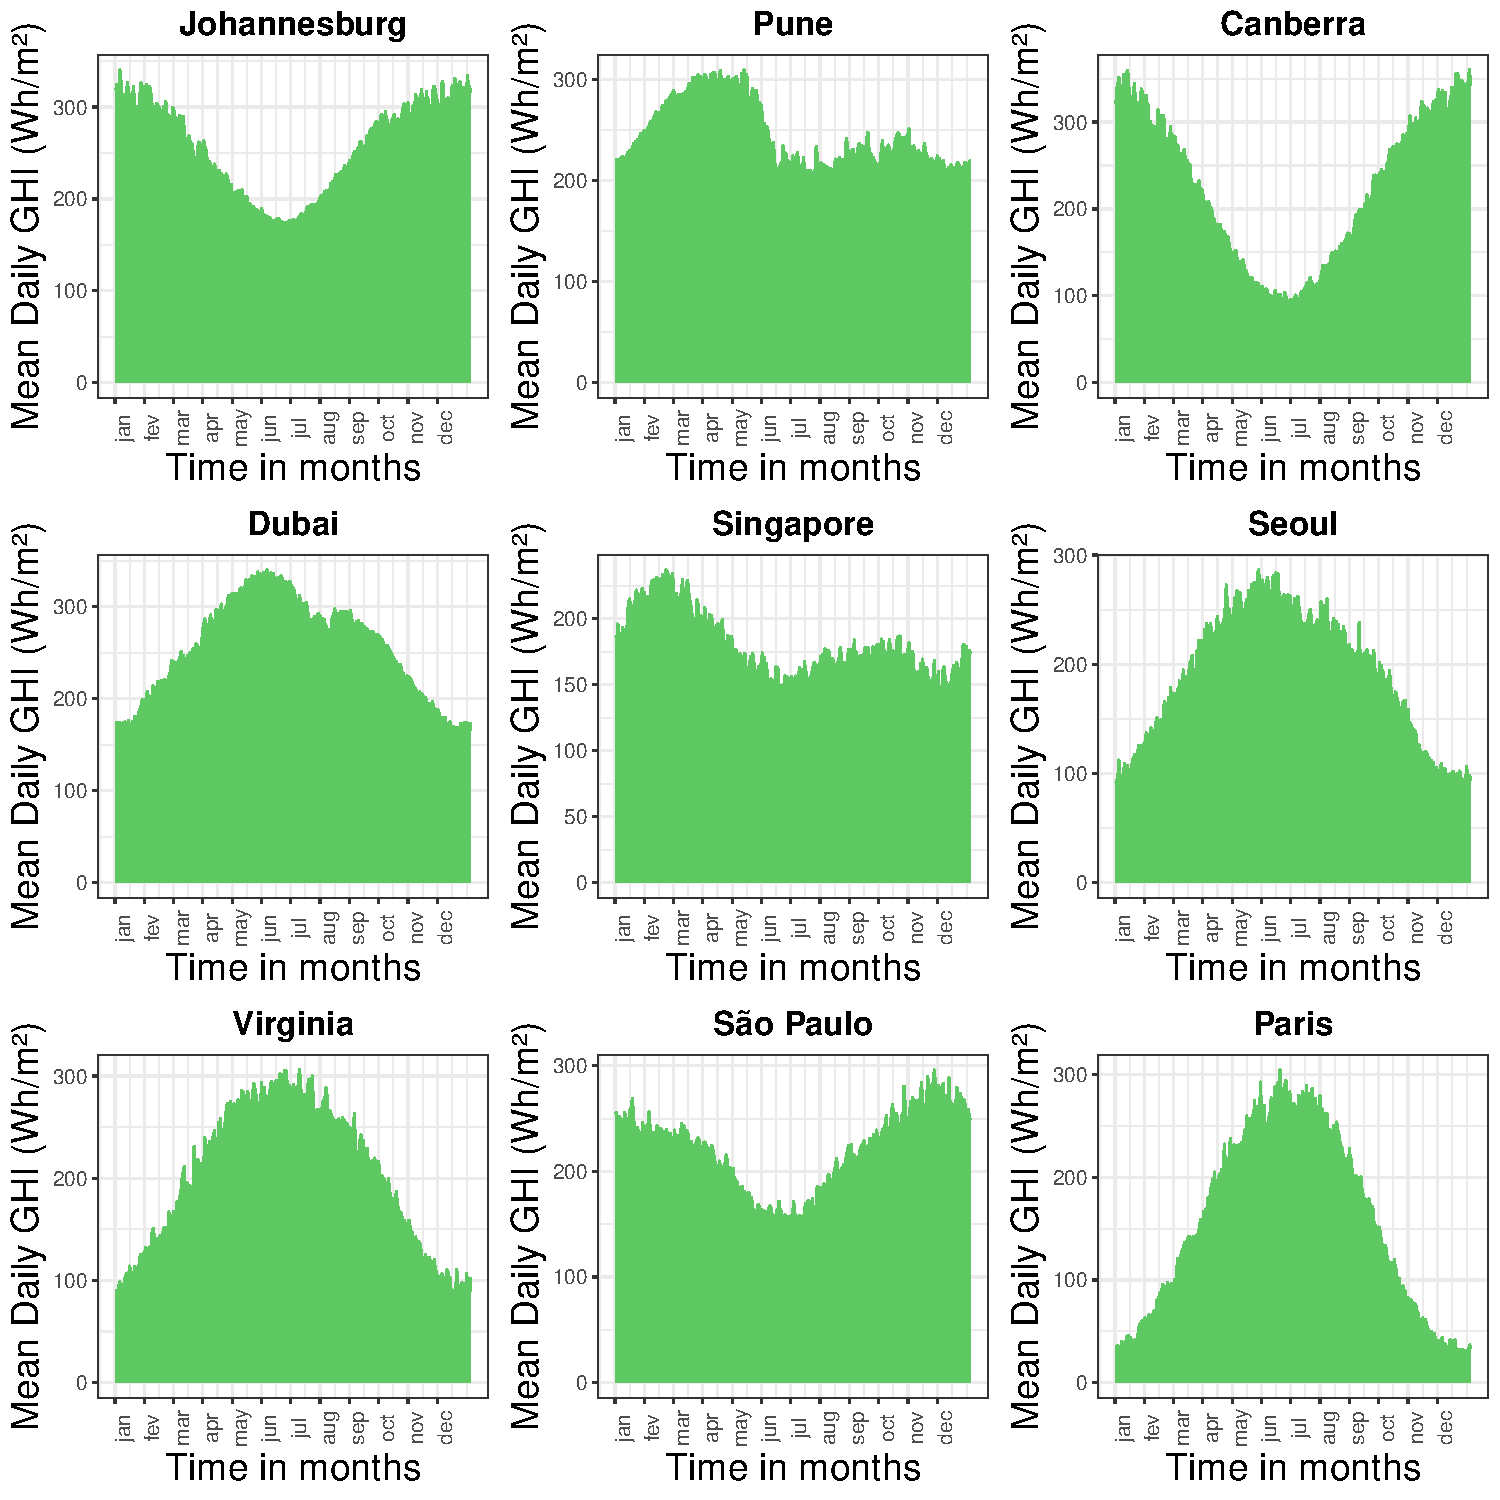
\epsfig{file = images/pv_daily_ghi_avg.pdf, width = .8\linewidth}}
   \caption{Average solar irradiation from 1980 to 2019 per location.}
  \label{fig:pv_ghi_avg}
\end{figure}

For the \ch{CO2} emissions of the batteries and PV whole life-cycle, we used values from the National Laboratory of Renewable Energy (NREL) of the United States that performed an analysis with over 3000 published studies on the life-cycle of renewable infrastructures \cite{nrel_lifecycle_2021}: $43 g\,\ch{CO2}-eq.Wh^{-1}$ for the PVs and $33 g\,\ch{CO2}-eq.Wh^{-1}$ for the Lithium-Ion batteries.

\subsubsection{Results}

Table~\ref{tab:emissions_LCA} presents the \ch{CO2} emissions of considering the whole life cycle in comparison with considering only the one from the manufacturing. As expected, the total \ch{CO2} emissions are higher (around 8\% of increase) since now the whole life cycle of the renewable infrastructure is taken into account. 

\begin{table}[!ht]
  
\caption{Total emissions for the different scenarios.}\label{tab:emissions_LCA} \centering

\begin{tabular}{|l|r|}
  \hline
  \textbf{Scenarios} & \textbf{Emissions ($t\,\ch{CO2}-eq$)}   \\
  \hline  
    \ch{CO2} from manufacturing   & 34559.03    \\  
  \hline
    \ch{CO2} from the whole life cycle       & 37778.79     \\
  \hline
  
\end{tabular}
\end{table}


\section{Including wind turbines to the renewable infrastructure}

In this section, we will evaluate the impact adding other renewable power source: wind turbines, and to what extent they complement the photovoltaic power production to reduce the total emissions of the cloud federation operation, in particular during the night and seasons with lower solar irradiation as the winter.

\subsection{Updates in the model}

We consider a new variable $WT^d$ that represents how much wind turbines will be built at each DC location. The number of wind turbines (WT) is an integer number (we cannot produce 1.2 WT for example). However, to avoid increasing the computational complexity of the LP by including integer variables, we made a relaxation in our modeling to allow the WT variable to be linear. 

The power production of the $WT^d$ wind turbines at location of data center $d$ at instant $k$ ($Pwt^d_{k}$) is modeled by Equation~\ref{eq:wt_power_prod}, where $V^d_k$ is the wind speed at location of data center $d$ at instant $k$; $Vici$ is the \textit{cut in} wind speed, that is, the wind turbines start producing power when the wind speed is greater or equal to $Vici$; $Vco$ is the \textit{cut out} wind speed, that is, the wind turbines stop producing power when the wind speed is greater than $Vco$; $Pr$ is the WT rated power production in W; and $Vr$ is the speed where the WT starts producing $Pr$ power. This model is based from \cite{HADDAD2021100505}.

\begin{equation} \label{eq:wt_power_prod}
Pwt^d_{k} = WT^d \times \left\{ 
  \begin{array}{ c l }
    0   & \quad \textrm{if } V^d_k \leq Vici \\
    Pr \times \frac{V^d_k - Vici}{Vr - Vici}  & \quad \textrm{if } Vici < V^d_k \leq Vr \\
    Pr  & \quad \textrm{if } Vr < V^d_k \leq Vco \\
    0  & \quad \textrm{if } Vco < V^d_k \\
  \end{array}
\right.
\end{equation}


To model the carbon footprint of the wind turbines, its whole life cycle also needs to be taken into account. Equation~\eqref{eq:fp_using_wt} models the footprint of using the WT at location of data center $d$ at instant $k$, where $wtCO2LC$ is the input that represents its emissions for the life cycle ( in $g\,\ch{CO2}-eq.Wh^{-1}$).

\begin{equation}\label{eq:fp_using_wt}
   FPwt^d_k =  wtCO2^d \times Pwt^d_{k}\times \Delta t
\end{equation}

Given that we are using an additional renewable power infrastructure, it is also necessary to update the model of the renewable power production on DC $d$ at instant $k$. Equation~\eqref{eq:new_pv_power} and Equation~\eqref{eq:new_renewable_power} models that the renewable power can be originated from both the PVs and WT.

\begin{equation} \label{eq:new_pv_power}
    Ppv^d_{k}= I^d_k \times Apv^d \times \eta_{pv}
\end{equation}

\begin{equation} \label{eq:new_renewable_power}
    Pre^d_{k}= Ppv^d_{k} + Pwt^d_{k}
\end{equation}

Finally, the objective function also needs to be modified in order to include the carbon emissions of using WTs. Equation~\ref{eq:new_obj_co2} models the new objective function.

\begin{equation} \label{eq:new_obj_co2}
  \text{minimize }\sum_{k=0}^{K-1} \sum_{d=1}^D ( FPgrid^d_k +  FPpv^d_k +  FPwt^d_k + FPbat^d_k) 
\end{equation}

\subsection{Experiments}

\subsubsection{Settings}

The cloud infrastructure, the workload, grid emissions, and the execution environment are the same as in Section \ref{sec:settings_ccgrid}. The solar irradiation values, and emissions from PV panels and batteries are the same as Section \ref{sec:ex_lca_pv}. For the \ch{CO2} emissions of the wind turbines, it is considered that it emits $13 g\,\ch{CO2}-eq.Wh^{-1}$ taking into account its life cycle. The source for the values was the same as in Section \ref{sec:ex_lca_pv}, the analysis from NREL that evaluated more than 3000 studies.

For the wind speed data, we used values from the ERA5 data-source \cite{era5_wind_2022}. They provide values for the 100m v-component of wind (air horizontal speed towards the east) and 100m u-component of wind (air horizontal speed towards the north). To transform these values into wind speed, we need to execute the following computation using the Pitagora's theorem: $ w_s = \sqrt{ v^2 + u^2} $, where $w_s$ is the wind speed, $u$ the value of the u-component and $v$ the value of the v-component.

\subsubsection{Results}

To evaluate the impact of including WT, we compare the sizing for using only PVs and batteries and using PV, batteries and WT. Table~\ref{tab:total_wind_and_pv_co2} presents the results in terms of total emissions when also considering the wind as renewable, we observe a reduction of approximately 6\% in comparison with the scenario where no WT is used and renewable energy is only produced by the PVs. 

\begin{table}[H]  
  \caption{Total emissions (tons of \ch{CO2} for different scenarios }\label{tab:total_wind_and_pv_co2} \centering  
  \begin{tabular}{|l|r|}
  \hline    
  \textbf{Scenario} &   \textbf{Total \ch{CO2} emissions (tons)} \\
  \hline    
  PV + Bat + WT + Grid  & 24895.74 \\    
  \hline
  PV + Bat + Grid       & 37778.79 \\    
  \hline
\end{tabular}  
\end{table}

Table~\ref{tab:results_wt} presents the number of WTs  built at each location. 

\begin{table}[H]
  
  \caption{Computed number of WT for each location}\label{tab:results_wt} \centering

  \begin{tabular}{|l|r|}
   \hline
    
  \textbf{Location} &   \textbf{Number of WT} \\
  \hline
  Johannesburg & 56.31   \\
  \hline
  Pune  & 25.42 \\
  \hline
  Canberra  & 75,31 \\
  \hline
  Dubai   &  75.51  \\
  \hline
  Singapore & 35.03  \\
  \hline     
  Seoul    & 111.25  \\
  \hline
  Virginia   & 39.19 \\
  \hline
  São Paulo   & 91.45 \\
  \hline 
  Paris    &    22.44 \\
  \hline
    
\end{tabular}  
\end{table}


To assess the impact of including the WT regarding the sizing of both PV and batteries, we present in Figure~\ref{fig:wind_bat} and Figure~\ref{fig:wind_pv}  the dimensioning for both equipment considering and not considering manufacturing WT. 

\begin{figure}[H]
  \centering
  {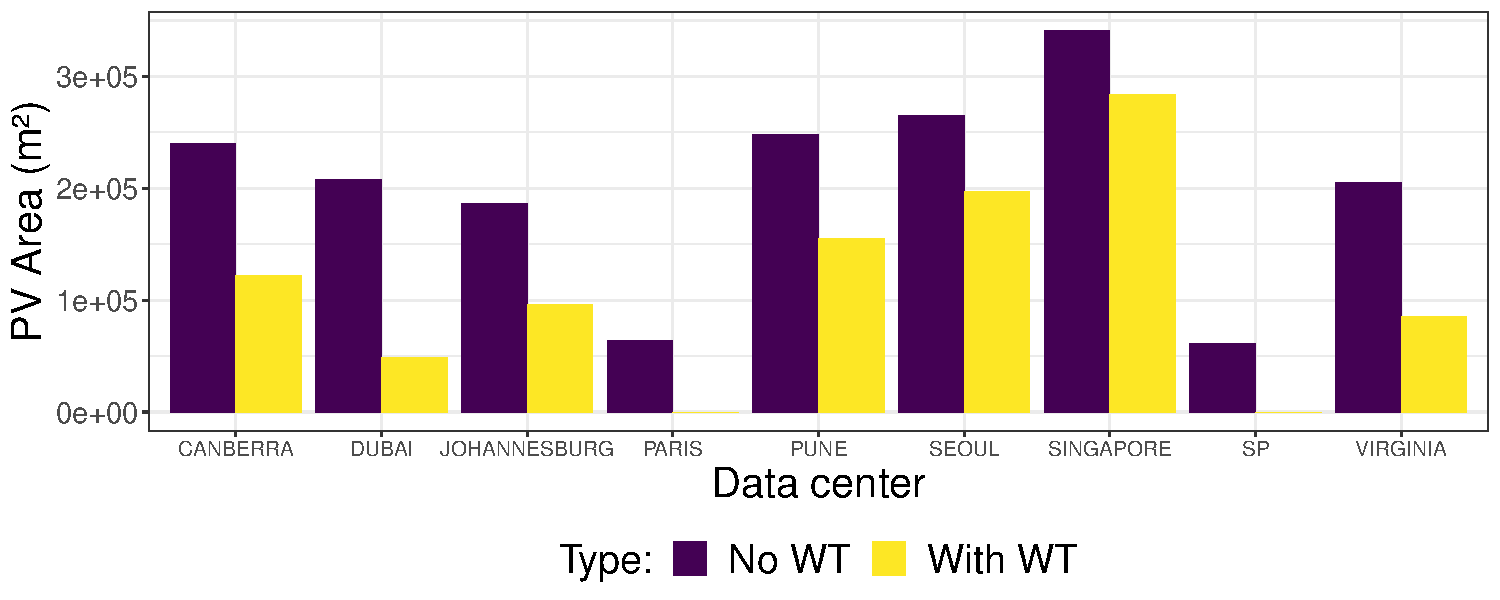
\epsfig{file = images/pv_sizing_after_wt.pdf, width = .8\textwidth}}
  \caption{PV Area sizing when the WT are and are not included }
  \label{fig:wind_pv}
\end{figure}


\begin{figure}[H]
  \centering
  {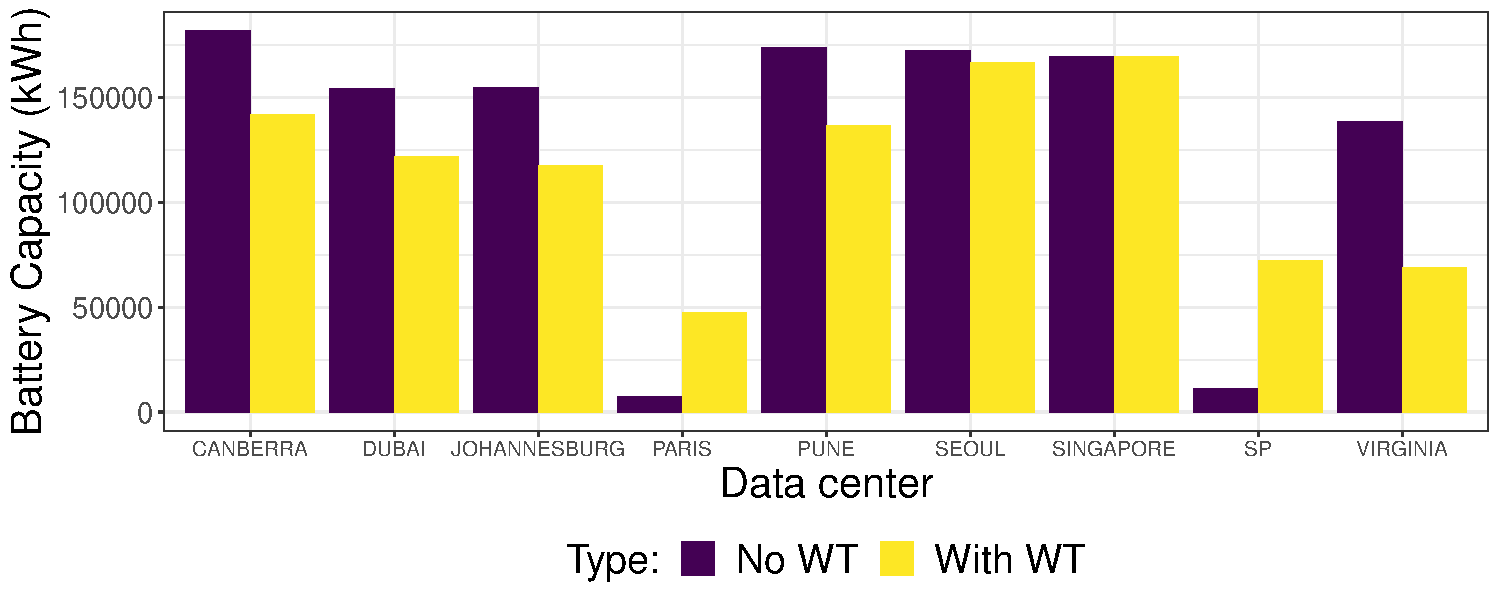
\epsfig{file = images/bat_sizing_after_wt.pdf, width = .8\textwidth}}
  \caption{Battery capacity sizing when the WT are and are not included }
  \label{fig:wind_bat}
\end{figure}

\section{Validating sensibility of the Linear Program to  uncertainties}

To assess the sensibility of the linear program to the inputs, we will evaluate it considering different scenarios in terms of solar irradiation, wind speed and grid emissions data. Regarding the intermitency of solar irradiation, there is no necessary modifications to be made in the model itself, the important point is which input data will be used for the sizing process.

Given the presence of low-carbon intensive sources in some countries, the emissions of the local electricity grid is not static all over the year, for example, regions that have access to solar energy have a lower grid footprint during the day. Some countries provide access to fine-grain information of its electricity mix in real time or historical data in the form of time series. However, obtaining data for all the locations is not an easy process: not all the locations provide this information, or they provide with different time granularity (day, hour, month), historical data with different durations (for example only the last 6 months), or only real time values. For modeling the variation in grid emissions is necessary to update the model, and in the next section we present the modifications.

\section{Updates in the model}

To model this variation in the emissions of the electricity grid, we need to change this input to be a time series. For the locations where data is not available at fine-grain, hour by hour for example, a pre-processing of the data is needed, for example, if the region it only provides daily data, one can assume that for the 24 hours of the day the grid emissions  will be the same value. It is also necessary to change the model, and Equation~\eqref{eq:fpgrid_timeseries} represents this modification where $gridCO2^d_k$ is the new input for the grid emissions with one value for each time slot $k$.


\begin{equation} \label{eq:fpgrid_timeseries}
FPgrid_k^d = Pgrid_k^d\times \Delta t \times gridCO2^d_k
\end{equation}

\subsection{Experiments}

\subsubsection{Settings}

The cloud infrastructure, the workload, grid emissions, and the execution environment are the same as in Section  \ref{sec:settings_ccgrid}. To evaluate the sensibility of the sizing process considering the solar irradiation data, that is intermittent, we perform the sizing process using the solar irradiation from 30 years (1980 to 2009), that is, for each year the corresponding irradiation data is used for the sizing process, generating a total of 30 instances. To isolate only the effect of the solar irradiation in the sizing process, all the other values are fixed for the 30 instances (workload, parameters, \ch{CO2} emissions from using the grid and manufacturing the renewable infrastructure).


The data for simulating the solar power production --- Global Solar Horizontal Irradiation (in Wh/m$^{2}$) --- was collected from the MERRA-2 project~\cite{GELARO2017MERRA2}, since it provides information for anywhere on earth.



In the experiment section we will present the results of considering the average and median irradiation of 30 years (PV module expected life time) and how the sizing will perform in the future, considering the long life time of the renewable infrastructure and the difficulty to predict climate conditions. To assess the results, we will compare with the optimal solution, that is, the solution that knows in advance all the climate condition of the next years.

 \begin{figure}[!htbp]
  \centering
   {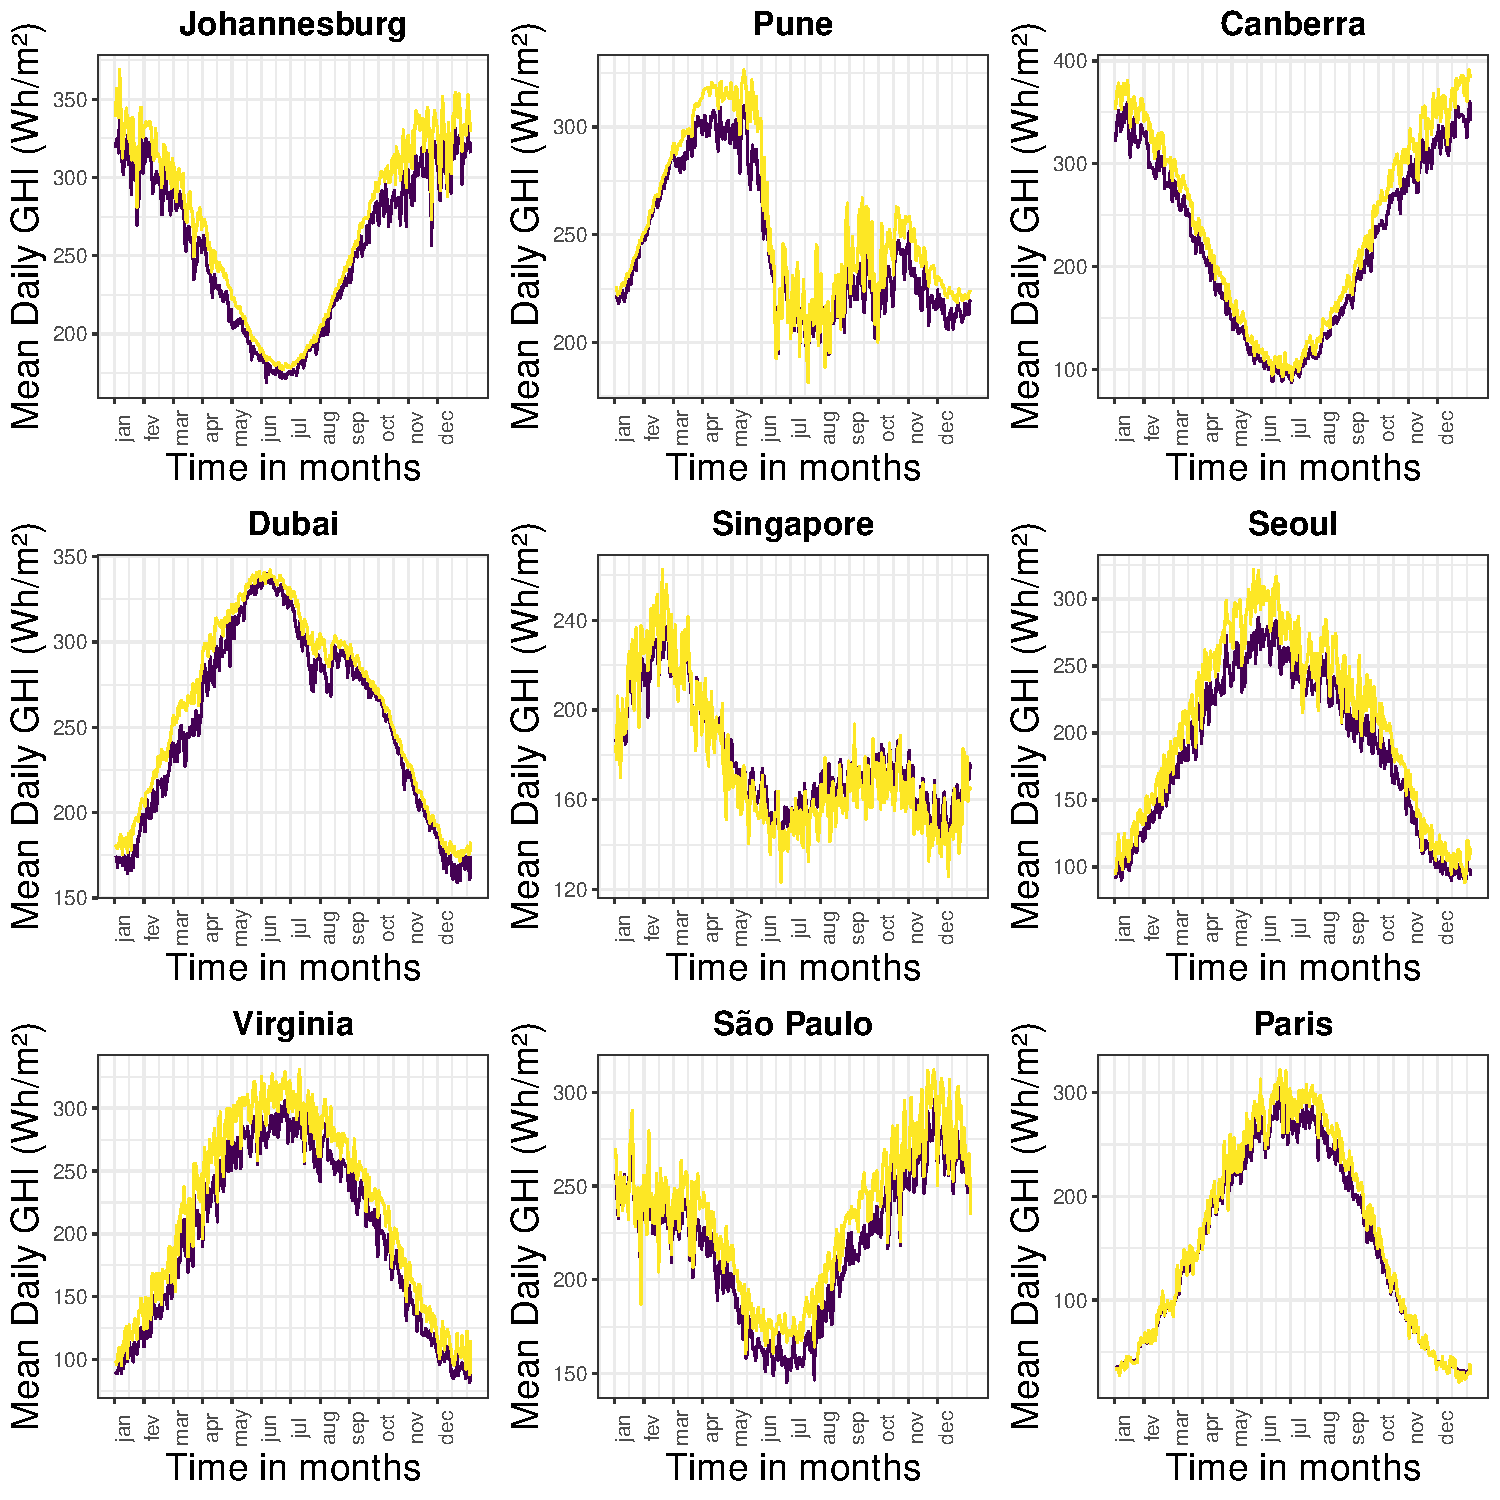
\epsfig{file = images/pv_daily_ghi_avg_median.pdf, width = \linewidth}}
   \caption{Different values for the solar irradiation input from 1980 to 2019. The data in yellow represents the median and in purple the average of the 30 years. }
  \label{fig:pv_ghi}
\end{figure}




Computing the optimal area of PV and batteries can also be considered as a type of forecasting, given the long life time of the equipments (30 years for PVs and 10 years for batteries) and the uncertainty about the climate conditions during the life time of the renewables infrastructure. In Figure~\ref{fig:pv_boxplots} and Figure~\ref{fig:bat_boxplots}, we showed only the values for the optimal sizing of each year, and when the irradiation is known. The DC operator is interested in the sizing for the future, that is, the following years where the renewable infrastructure will be used. Predicting the solar irradiation data that a region will receive is not a simple task, and it also involves predicting the weather, since clouds can affect the amount of solar irradiation received by the region. 


To evaluate the results of the sizing and which solar irradiation data should be used, we will evaluate it for a duration of 10 years. 

We use the solar irradiation data for 30 years to generate the sizing (from 1980 to 2009) and evaluate the resulted sizing when operating the cloud federation for the next 10 years (from 2010 to 2019), using the new solar irradiation values.

The sizing process was performed for two scenarios considering the 30 years of solar irradiation data: in the first, the average solar irradiation for each hour, and in the second, using the median.

The baseline, was the optimal sizing for the 10 years (2010 - 2019) where all the solar irradiation data is know in advance.




In order to evaluate what is the impact of using this fine-grain information of the grid \ch{CO2} on the sizing process, we perform the sizing using the time series provided by Electricity Map for the locations: Pune, Canberra, Seoul, Virginia, São Paulo and Paris. These time series have the span of one year, and one value for each hour. For the regions Johannesburg and Singapore, the information of the \ch{CO2} emissions was in the granularity of months. Therefore, we generated a time series with a total duration of one year with the same value of \ch{co2} per hour for each corresponding month that we have the grid \ch{co2} emissions. For Dubai, we only found data for the year average grid \ch{co2} emissions, and we generated a time series in which the grid emissions is fixed for every hour. Considering the selected locations for the DCs listed before, Table~\ref{tab:grid_emissions_hist} presents the data that was found.

\begin{table}[H]
  
\caption{Comparison of local electricity grid access to information }\label{tab:grid_emissions_hist} \centering
  
  \begin{tabular}{|l|r|r|r|}
  \hline
    
  \textbf{Location} &   \textbf{Granularity} & \textbf{Span} & \textbf{Source} \\
  \hline
  Johannesburg & month & year & ElectricityMaps  \\
  \hline
  Pune  & hour & year & ElectricityMaps  \\
  \hline
  Canberra  & hour &  year & ElectricityMaps \\
  \hline
  Dubai    & year & year & https://1p5ndc-pathways.climateanalytics.org/  \\
  \hline
  Singapore & month & year & ElectricityMaps \\
  \hline     
  Seoul     & hour & year & ElectricityMaps \\
  \hline
  Virginia  &  hour & year & ElectricityMaps \\
  \hline
  São Paulo & hour & year  & ElectricityMaps \\
  \hline 
  Paris     & hour & year  & ElectricityMaps  \\
  \hline


\end{tabular}  
\end{table}

We compared the results of using the grid emissions hour by hour with using one value with the average of the year. Table~\ref{tab:co2_grid_granularities} presents the results. For all the scenarios, using the  year average grid \ch{CO2} resulted in higher emissions, but the difference is very small --- less than 1\%.

% bom para os casos em que o dado eh dificil de encontrar com baixa granularidade, entao esse com a media anual eh mais ok ...




\begin{table}
  
  \caption{Average emissions (in $g\,\ch{CO2}-eq.kWh^{-1}$) from using the regular grid at the different years.}\label{tab:carbonfootprint} \centering
  \begin{tabular}{|l|r|r|r|r|}    
  \hline   
  \textbf{Location} &  \textbf{2021} & \textbf{2020} & \textbf{2019} & \textbf{2018}\\
  \hline
  Johannesburg & 700.66 & 700.66 & 700.66 & 700.66  \\
  \hline
  Pune & 728.15 & 724.04 & 726.43 & 723.83     \\
  \hline
  Canberra & 655.36 & 692.23 & 712.43 & 728.21\\
  \hline
  Dubai & 530.00  & 530.00 & 530.00 & 530.00     \\
  \hline
  Singapore & 491.01 & 491.01 & 491.01 & 491.01 \\
  \hline     
  Seoul & 490.60 & 490.15 & 490.73 & 490.90     \\
  \hline
  Virginia  & 435.25 & 415.14 & 447.98 & 453.40 \\
  \hline
  São Paulo &  172.54 &  103.47 & 108.95 &  105.21 \\
  \hline 
  Paris &  63.48  & 62.99 & 61.62   & 60.00   \\
  \hline  

\end{tabular}  
\end{table}


\subsubsection{Results}

Table \ref{tab:co2_10y} presents the results in terms of \ch{CO2} emissions. We observe that these simple forecasting techniques already have a good precision value, up to 2\% difference compared to the optimal scenario. Using a simple method is also interesting because of the computational costs of the computation, resulting in a smaller \ch{CO2} footprint for the sizing process by itself.

\begin{table}
  \caption{Emissions (in kt \ch{CO2}-eq) for the different scenarios} \centering
    \label{tab:co2_10y}
      \begin{tabular}{|l|r|r|}        
        \hline        
        \textbf{Sizing Scenario} &  \textbf{Emissions } & \textbf{Diff. to baseline (\%) } \\
        \hline        
        Optimal sizing 2010 - 2019  &       296.367 & - \\
        \hline     
        Average irrad.  1980 - 2009  & 301.237 &  1.62 \\
        \hline
        Median irrad. 1980 - 2009  &        304.489 & 2.66 \\
        \hline        
      \end{tabular}      
    \end{table}
   
Furthermore, there was an increase of 0.25\% in \ch{CO2} emissions. Figure~\ref{fig:pv_grid_co2_sizing} and \ref{fig:bat_grid_co2_sizing} illustrates the difference in the sizing, both for PVs and batteries, respectively, when we use this different granularity for grid \ch{CO2} emissions data.


\begin{table}[H]  
  \caption{Total emissions (tons of \ch{CO2}) for different scenarios }\label{tab:co2_grid_granularities} \centering
  
  \begin{tabular}{|l|r|r}
   \hline
    
  \textbf{Scenario} &   \textbf{Total \ch{CO2} emissions (tons)} \\
  \hline
  Fine grain grid emissions data & 30911.03 \\
  \hline
  Average of the year grid emissions data & 30831.14 \\
  \hline

\end{tabular}  
\end{table}


\begin{figure}[H]
  \centering
  {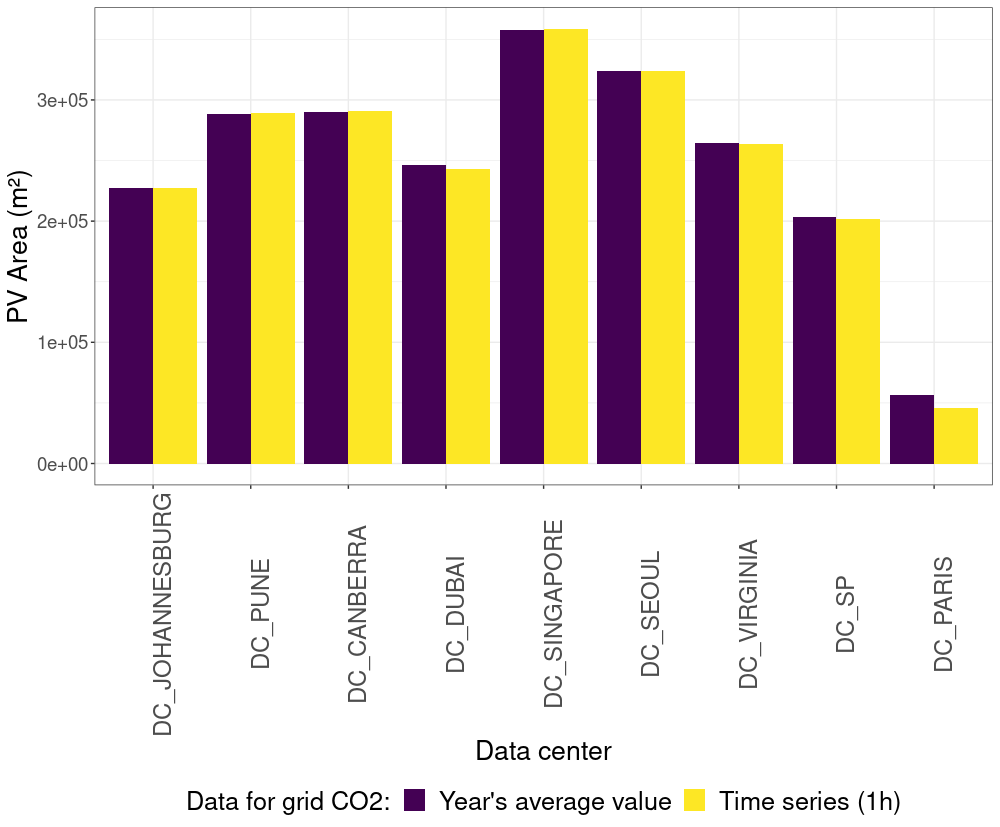
\epsfig{file = images/sizing_pv_grid_co2.png, width = \textwidth}}
  \caption{PV sizing with different granularity for grid \ch{CO2} emissions data}
  \label{fig:pv_grid_co2_sizing}
\end{figure}


\begin{figure}[H]
  \centering
  {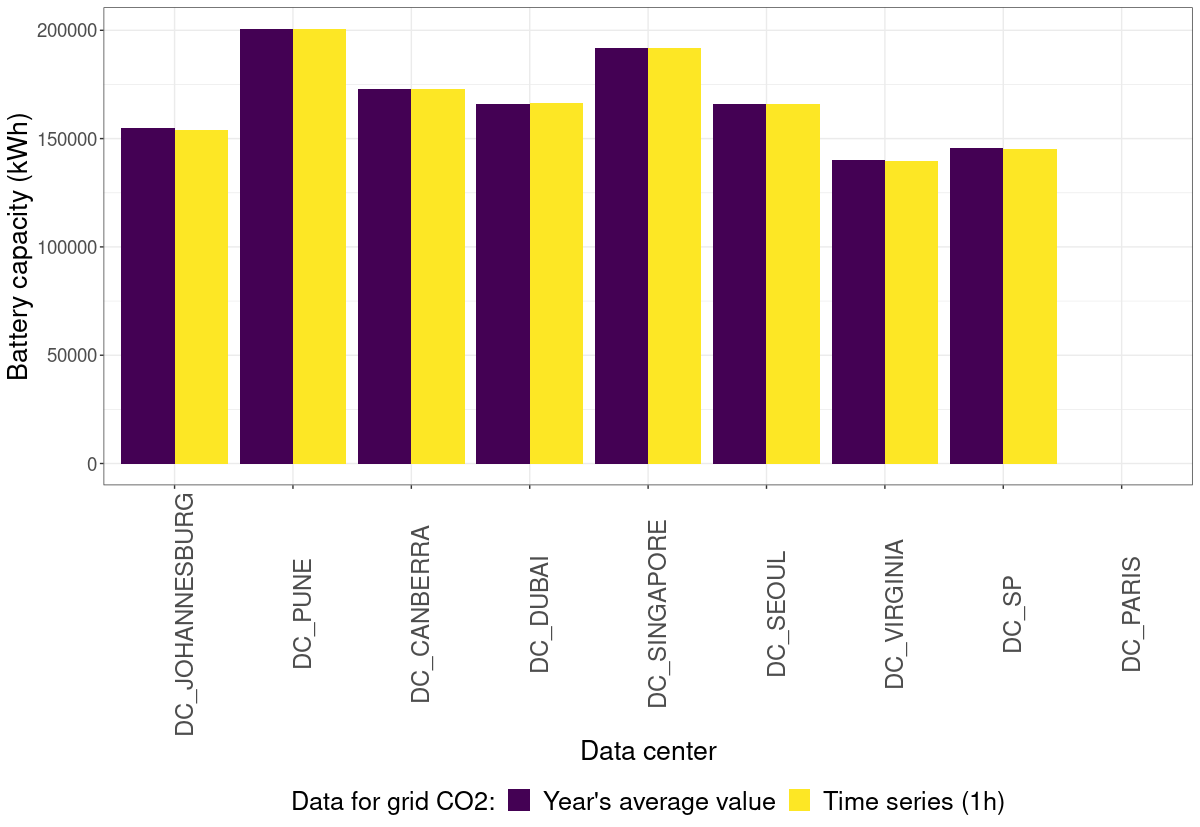
\epsfig{file = images/sizing_bat_grid_co2.png, width = \textwidth}}
  \caption{Battery sizing with different granularity for grid \ch{CO2} emissions data }
  \label{fig:bat_grid_co2_sizing}
\end{figure}



\begin{table}[H]

  \caption{Difference in total emissions (tons of \ch{CO2}) between using avg. co2 of the year vs co2 per hour for the different years. Values greater than zero represents that using co2 values per hour increased the total emissions.}\label{tab:co2_grid_granularities_years} \centering

  \begin{tabular}{|l|r|r}
    \hline
    
  \textbf{Year} &   \textbf{Difference (\%) in \ch{CO2} emissions} \\
  \hline
  2018 &   0.34 \\
  \hline
  2019 &   0.59 \\
  \hline
  2020 &   0.18 \\
  \hline
  2021 &   0.74 \\
  \hline

\end{tabular}  
\end{table}




In Figure~\ref{fig:pv_boxplots} we present a boxplot with the different values of the optimal sizing for the 30 years regarding the PV dimensioning, and in Figure~\ref{fig:pv_boxplots} regarding the battery dimensioning. For both figures, the sizing was made using the irradiation of a single year (from 1980 to 2019). We observe a high difference for the PV area for some locations (Canberra, Seoul, Virginia, and the highest difference was in Singapore). From the figures it is clear that using solar irradiation just for a single year is not enough to deal with the intermittency of irradiation, and the PV area can be very different depending on the year selected for the sizing process. For the batteries, the difference in the sizing is small because they are used mostly for night computations.


\begin{figure}[H]
  \centering
  {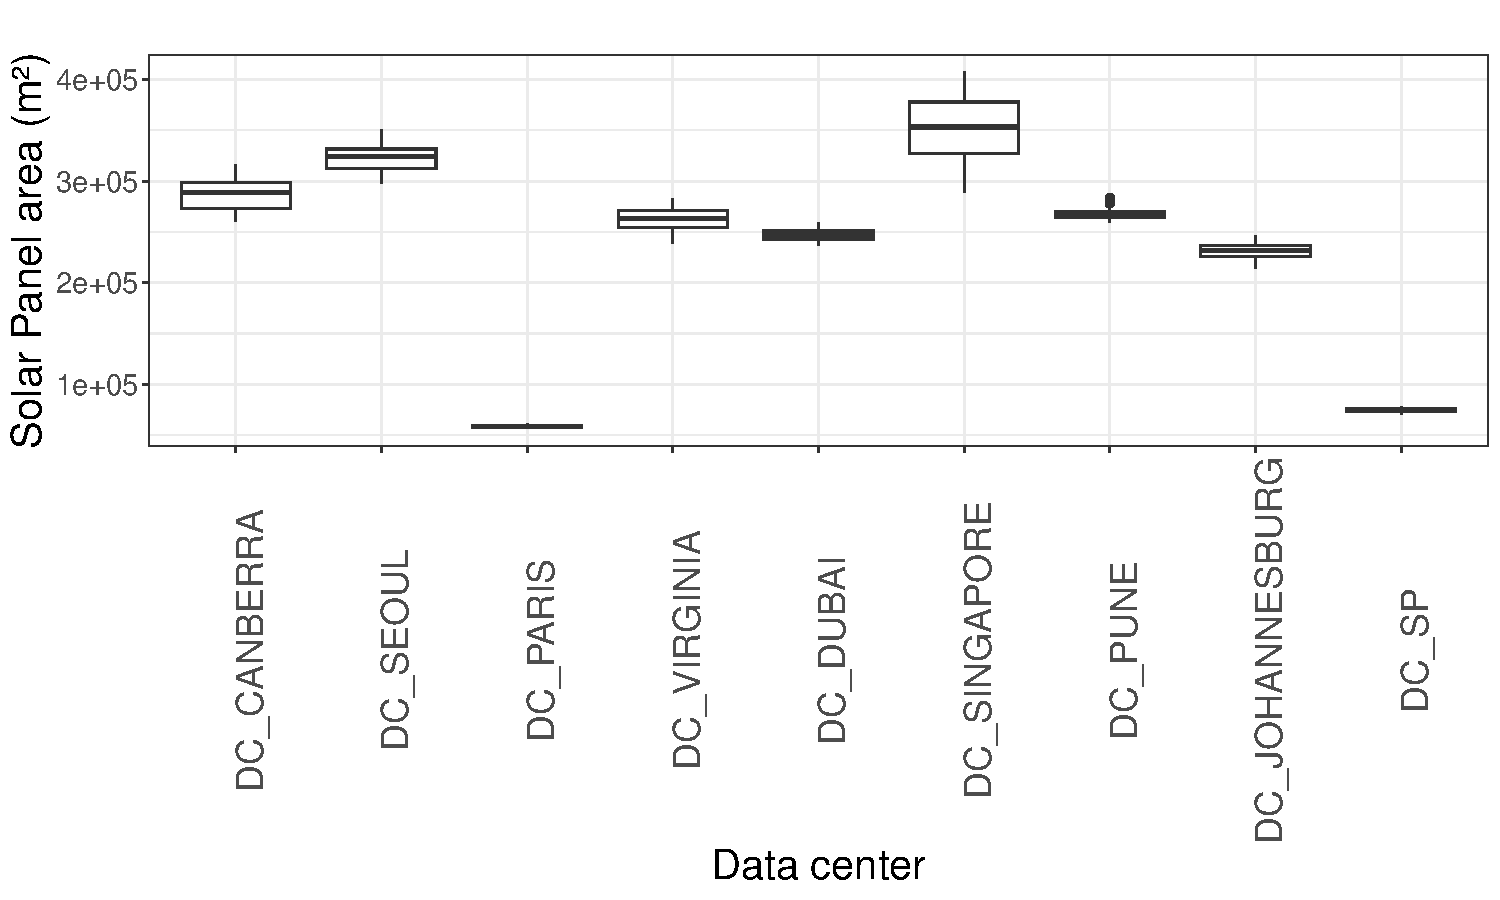
\epsfig{file = images/pv_boxplots_1980_2009.pdf, width = .8\textwidth}}
  \caption{Different PV sizing using irradiation from 30 years (1980 - 2009).}
  \label{fig:pv_boxplots}
\end{figure}


\begin{figure}[H]
  \centering
  {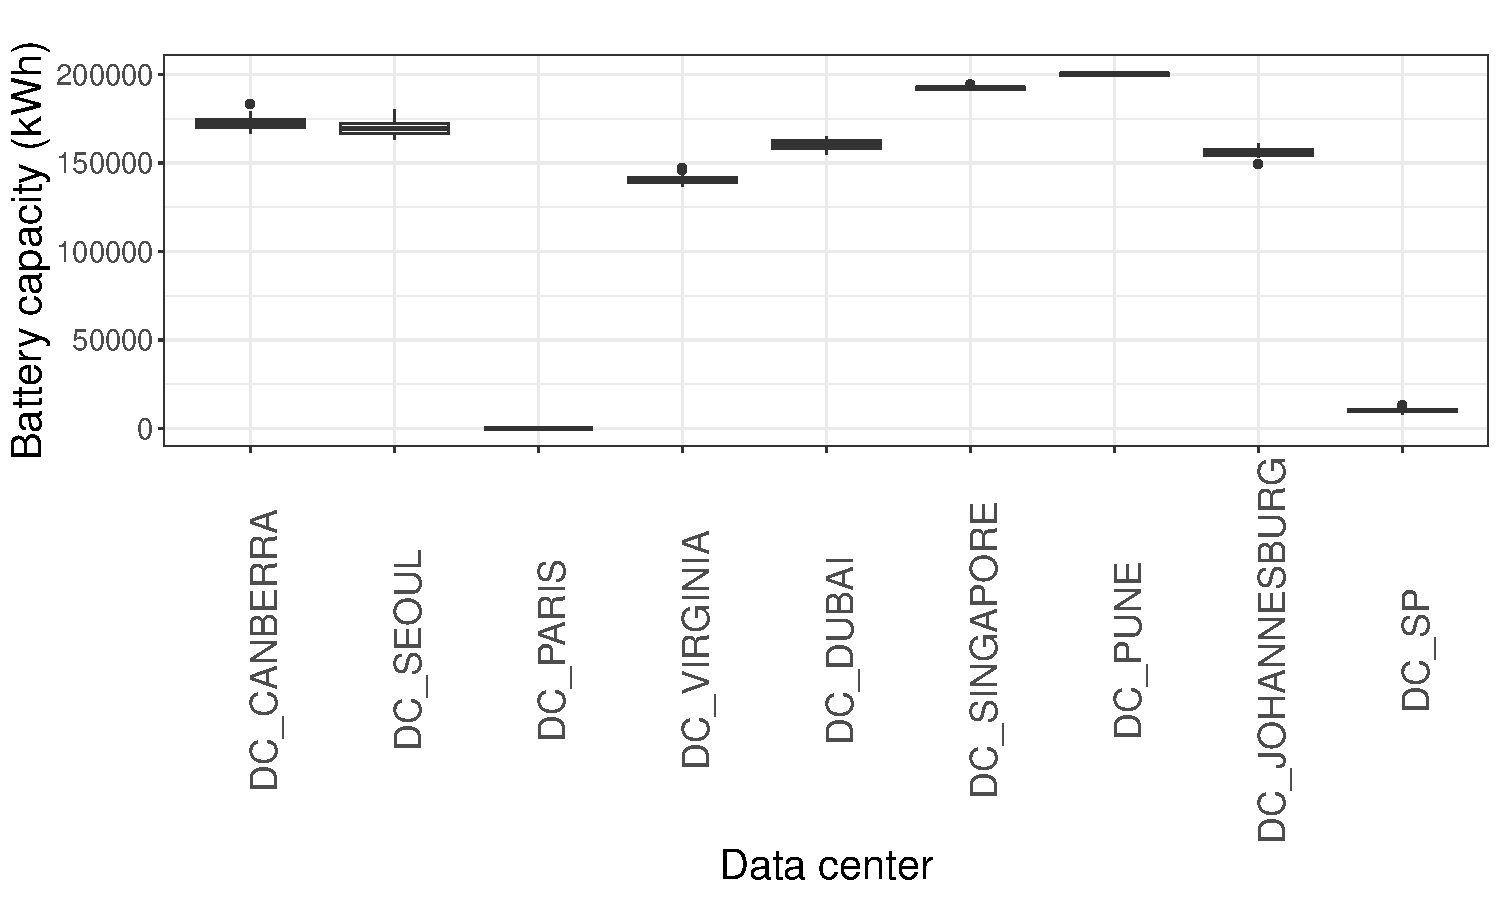
\epsfig{file = images/bat_boxplots_1980_2009.pdf, width = .8\textwidth}}
  \caption{Different battery sizing using irradiation from 30 years (1980 - 2009).}
  \label{fig:bat_boxplots}
\end{figure}



\section{Flexibility in the scheduling to reduce carbon emissions}

\section{Updates in the model}

Suppose that we have the flexibility to delay $\alpha$ percent of workload up to $\beta$ time slots. We need two new variables to model this new feature: $alloc^d_k$ that represents the workload allocated to the data center $d$ that will start executing at the time slot $k$; and $delay_{k,i}^d$, which represents the workload of data center $d$ that can be delayed from time slot $k$ up to $\beta$ time slots ($i$ is the index of list of size $\beta$ for the delayed workload).

This feature also requires new restrictions. Equation~\eqref{eq:alpha} models the flexibility of allowing $\alpha$ percent of the workload to be delayed, where $W_k$ is the input that represents the total CPU cores demand to execute the workload at time slot k.


\begin{equation} \label{eq:alpha}
   \sum_{d=1}^D  \sum_{i=1}^{\beta} delay_{k,i}^d \leq  \alpha   \times W_k
\end{equation}


Equation~\eqref{eq:beta} models the flexibility to delay the workload up to the next $\beta$ time slots and ensure that all the workload will be executed:


\begin{equation} \label{eq:beta}
       \sum_{d=1}^D    (  alloc_k^d +    \sum_{i=1}^{\beta} delay_{k,i}^d  ) = W_k  
     \end{equation}

The allocated workload at a time slot k, and the delayed workloads from the previous k - $\beta$ time slots need to respect the data center servers CPU core capacity. Equation ~\eqref{eq:beta_capacity} models this restriction. 

\begin{equation} \label{eq:beta_capacity}
\sum_{d=1}^D    (  alloc_k^d  +    \sum_{i=k-\beta}^{k-1} delay_{  i ,  k-i  }^d  )  \leq C_d 
\end{equation}

\subsection{Experiments}

\subsubsection{Settings}

The cloud infrastructure, the workload, grid emissions, and the execution environment are the same as in Section  \ref{sec:settings_ccgrid}. In order to evaluate only the impact of the flexibility of the scheduling in reducing the carbon emissions, all the other parameters are fixed: workload, solar irradiation (average from 1980 to 2019), wind speed (average from 2000 to 2020) area of PV panels and the capacity of the batteries, number of wind turbines, power consumption of servers and network devices, and so on. We will present an evaluation for delaying 10\% up to 50\% of the workload --- $\alpha$ values of 0.1, 0.2, 0.3, 0.4 and 0.5 --- for the period of one hour up to one week --- $\beta$ values of 1h, 6h, 12h, 24h, 48h, 96h, 120h.

\subsubsection{Results}

 The results of the experiments in terms of reduction of \ch{CO2} emissions are presented in Table \ref{tab:flex_scheduling}.

  \begin{table}[H]
    \caption{Initial results regarding the relative total carbon emissions reduction (in \%) for different values of $\alpha$ (how much of the workload to delay) and $\beta$ (how long to delay the workload).}\centering
    \label{tab:flex_scheduling}
    \begin{tabular}{|l|r|r|r|r|r|r|r|r|r|r|}
      \hline
      $\alpha$, $\beta$ &   \textbf{$ 1 h $} &   \textbf{$ 6 h $} &  \textbf{$ 12 h $} &  \textbf{$ 24 h $} &  \textbf{$ 48 h $} &  \textbf{$ 96 h$} &   \textbf{$ 120 h $} &   \textbf{$ 144 h$} &   \textbf{$ 168 h$}\\ 
      \hline
      10 \%   &  0.08 &  0.3 &  0.43 &  0.59 &  0.88 &  1.15 &  1.27 &  1.36 &  1.42 \\ 
      \hline
      20 \%   &  0.14 &  0.43 &  0.59 &  0.88 &  1.16 &  1.52 &  1.55 &  1.55 &  1.55 \\ 
      \hline
       30 \%   &  0.19 &  0.51 &  0.75 &  1.04 &  1.38 &  1.55 &  1.55 &  1.56 &  1.56 \\ 
      \hline
       40 \%  &  0.24 &  0.59 &  0.88 &  1.16 &  1.52 &  1.56 &  1.56 &  1.57 &  1.57 \\ 
      \hline
       50 \%   &  0.27 &  0.67 &  0.96 &  1.28 &  1.55 &  1.56 &  1.57 &  1.57 &  1.57 \\ 
      \hline
    \end{tabular}
  \end{table}

\section{ Monetary costs of reducing the carbon emissions}

On the previous sections we showed the results only in terms of the environmental impact of the cloud operation, now we will present the results in terms of monetary costs (in dolars) of operating the cloud platform and how much would it costs for the DC operator to reduce their environmental impact. This is also an important aspect, as the decision-makers wants their business to be lucrative.

\subsection{Updates in the model}

To perform this new analysis, we need some modification in our modeling. The first modification regards buying electricity from the regular grid, and it is modeled by Equation~\eqref{eq:pricegrid}, where $costGrid^d$ is an input that represents the costs of buying electricity at each location. 

\begin{equation} \label{eq:pricegrid}
 PriceGrid^d_k = Pgrid^d_k \times costGrid^d
\end{equation}

To measure the price of the electricity of the renewable sources, we can use the Levelized Cost of Energy (LCOE). This metric compares the total costs of manufacturing and operating the electricity infrastructure (for example the PV panel) with the total energy it can deliver in its life time, therefore the metric is in \$ per kWh. Similar to the \ch{CO2} emissions of renewable sources, the price will also be different per location, as the total amount of irradiation received differs.  Equation~\eqref{eq:pricepv} models the costs of consuming energy from the solar panels, where $PVLCOE^d$ represents the specific LCOE at the location of data center $d$. 

\begin{equation} \label{eq:pricepv}
  PricePV^d_k = PPV^d_k \times PVLCOE^d
\end{equation}

For the batteries, the metric Levelized Cost of Storage (LCOS) is similar to the LCOE, and it represents how much it costs to discharge energy of the battery considering all the costs in its lifetime. Equation~\eqref{eq:pricebat} models the costs of the energy used from the batteries using its LCOS as input ($BatLCOS$).

\begin{equation} \label{eq:pricebat}
   PriceBat^d_k = Pdch^d_k \times BatLCOS
\end{equation}


We can also modify our objective function to minimize the price of operating the cloud platform instead of its environmental impact, and Equation~\eqref{eq:objective_price} model this new objective.

\begin{equation} \label{eq:objective_price}
\text{minimize }\sum_{k=0}^{K-1} \sum_{d=1}^D PriceGrid^d_k  + PriceBat^d_k + PricePV^d+k
\end{equation}

\subsection{Experiments}

\subsubsection{Settings}

The cloud infrastructure, the workload, grid emissions, and the execution environment are the same as in Section  \ref{sec:settings_ccgrid}.

For the price of solar panel electricity, we use the tool ``Comparative Photovoltaic Levelized Cost of Energy Calculator'' from the National Renewable Energy Laboratory of the USA \cite{pv_lcoe_calc} --- version 2.0.0 of August 2021. This tool provide a detailed cost model for many parts of the PV panel, and the default values are adequate. For reproducibility purposes, Table \ref{tab:parameters_pv_LCOE} lists the values of the parameters used, and the only differences between the default values were for the parameters Service life, Performance Efficiency, and the Energy yield (that depends on the location where the PV module is installed). For the latter, the following values where considered: Canberra = 1934.0329615975024 ; Seoul  = 1648.08; Paris = 1346.32 ; Virginia = 1737.38; Dubai =  2215.17; Singapore = 1549.23; Pune =  2125.62 ; Johannesburg = 2238.52; and São Paulo =  1904.66.

\begin{table}[H]
  
  \caption{Parameters used in the LCOE PV calculator}\label{tab:parameters_pv_LCOE} \centering

  \begin{tabular}{|l|r|}
    \hline    
    \textbf{Parameter name} &   \textbf{Value} \\
    \hline
    Cell technology & mono-SI  \\
    \hline
    Package type  & glass-polymer backsheet \\
    \hline
    System type  & fixed tilt, utility scale \\
    \hline
    Inverter loading ration  & 1.5 \\
    \hline
    Front layer cost (USD/m²)   &  3.5 \\
    \hline
    Cell  cost (USD/m²)   &  22.20 \\
    \hline
    Back layer cost (USD/m²)   & 2.40 \\
    \hline
    Non-cell module cost (USD/m²)   &  13.60 \\
    \hline
    Extra component cost (USD/m²)   &  0 \\
    \hline
    Operations and Maintenance cost  (USD/kWDC/year)   &  3.5 \\
    \hline  
    Balance of system cost,power-scaling  (USD/W)   &  0.2 \\
    \hline  
    Balance of system cost,area-scaling  (USD/m²)   &  53.38 \\
    \hline  
    Performance Efficiency (\%) & 15.0  \\
    \hline
    Energy yield (kWh/kWDC) & specific per location \\
    \hline
    System degradation rate (\%/year)  & 1.0 \\
    \hline
    Service life (years) & 30 \\
    \hline
    Discount rate & 6.3 \\
    \hline
    

  \end{tabular}  
\end{table}

For the batteries, the metric Levelized Cost of Storage (LCOS) is similar to the LCOE, and it can represents how much it costs to discharge energy of the battery considering all the costs in its lifetime. We used values from a technical report of the US Department of Energy \cite{battery_lcos_2022}, where each kilowatt hour of energy discharged has a price of 20 cents. For the grid electricity prices, we used the source from Petrolprices.org. Finally, Table \ref{tab:price_electricity_sources} presents the cost in dolars per kWh of using the electrical grid and PV panels.

\begin{table}[H]
  
  \caption{Price of different sources of energy (USD per kWh) at each location }\label{tab:price_electricity_sources} \centering

  \begin{tabular}{|l|r|r|r|}
   \hline
    
  \textbf{Location} &   \textbf{Grid} & \textbf{PV}  \\
  \hline
  Johannesburg & 0.074 & 0.0385   \\
  \hline
  Pune      &  0.104   & 0.0406   \\
  \hline
  Canberra  & 0.331    &  0.0445  \\
  \hline
  Dubai   & 0.101      & 0.0390   \\
  \hline
  Singapore & 0.272    & 0.0557   \\
  \hline     
  Seoul      & 0.092   & 0.0525   \\
  \hline
  Virginia   & 0.150   &  0.0498  \\
  \hline
  São Paulo  & 0.144   &  0.0453  \\
  \hline 
  Paris      & 0.340   &  0.0643  \\
  \hline  

\end{tabular}
\end{table}

\subsubsection{Results}

Table~\ref{tab:total_price} illustrates the total costs for the data center operator considering multiple scenarios. The \textit{Minimum Costs} scenario refers to solving the LP using the objective of Equation~\eqref{eq:objective_price}; the \textit{Minimum \ch{CO2}} refers to solving the LP using  the objective of Equation~\eqref{eq:FPALL}; \textit{Only renewable infra} represents the case where the DC are autonomous and only use power produced from their local renewable infrastructure; and \textit{Only grid} represents the case where there is no renewable infrastructure in the DCs and they only use power from the local electricity grid.


\begin{table}[H]

  \caption{Total costs (millions of \$) for different scenarios }\label{tab:total_price} \centering
  
  \begin{tabular}{|l|r|}
   \hline
    
  \textbf{Scenario} &   \textbf{Total costs (millions of \$)} \\
  \hline
  Minimum cost (PV + Bat + WT + grid) & 36.926   \\
  \hline
  Minimum cost (PV + Bat  + grid)   & 37.889 \\
  \hline
  Minimum \ch{CO2} (PV + Bat + WT + grid)  & 45.667 \\
  \hline
  Minimum \ch{CO2} (PV + Bat + grid)   & 50.054 \\
  \hline
  Only renewable infra (PV + Bat + WT ) & 51.104  \\
  \hline     
  Only renewable infra (PV + Bat)     & 52.694 \\
  \hline
  Only grid   & 75.378\\
  \hline
  
\end{tabular}  
\end{table}


\begin{table}[H]

  \caption{Total emissions (tons of CO2 for different scenarios }\label{tab:total_co2_scenarios} \centering
  
  \begin{tabular}{|l|r|}
   \hline
    
  \textbf{Scenario} &   \textbf{Total CO2 emissions (tons)} \\
  \hline
  Minimum \ch{CO2} (PV + Bat + WT + grid)  & 27821.1\\
  \hline
  Minimum \ch{CO2} (PV + Bat + grid)   & 29541.7 \\
  \hline
  Only renewable infra (PV + Bat)     & 42316.25 \\
  \hline
  Minimum cost (PV + Bat + WT + grid) &  101170.9\\
  \hline
  Minimum cost (PV + Bat  + grid)   & 101930.9 \\
  \hline

\end{tabular}  

\end{table}


\subsection{Adding or replacing servers considering new generations }

In this section we show the necessary modifications in our modeling to evaluate the decision of manufacturing servers from new generations to match the cloud workload demand, considering that the servers also emits \ch{CO2} during its life time. It is assumed a long-term operation of the cloud federation (10 years for example) and that every year a new server is launched, and it will be made a decision to manufacture this new server to be added with the servers with the previous generations or to replace them.

\subsection{Updates in the model}

To model this approach, two new variables were created: $NS^d$, that represents the number of new servers to manufacture at data center $d$; and $REP_{gen}^d$, number of servers of the generation $gen$ to replace at data center $d$.

For replacing servers from previous generations, it is considered that the data center computational capacity in number of CPU cores cannot decrease, that is, the sum of the number of CPU cores of the new generation servers needs to be greater or equal to the number of the sum from the servers replaced. This constraint is modeled by Equation~\eqref{eq:dc_cpu_capacity}.

\begin{equation} \label{eq:dc_cpu_capacity}
 NS^d \times cpucores_{newgen} \geq \sum_{oldergen}  REP_{oldergen}^d \times cpucores_{oldergen}
\end{equation}

The number of servers replaced of a generation cannot be greater than the number of servers of this generation that exists in the DC ($ES_{gen}^d $). The value of  $ES_{gen}^d $ is extracted from the solution of the previous year. Equation~\eqref{eq:rep_only_existing_servers} models this constraint.

\begin{equation} \label{eq:rep_only_existing_servers}
 REP_{gen}^d \leq ES_{gen}^d 
\end{equation}


Given that a data center may have servers of different generations, it is also necessary to update the models regarding the workload and the power consumption. Now we have a variable $w_{k,gen}^d$ that represents the workload that is executed on the servers of a generation $gen$ at the data center $d$ during time slot $k$. We have two constraints for this variable: one for the servers that already exists in the DC, and another for the new servers that will be manufactured in the DC. Equation~\eqref{eq:workload_gen} models this constraint.


\begin{equation} \label{eq:workload_gen}
w_{k,gen}^d \leq   \left\{ 
  \begin{array}{ c l }
    (ES_{gen}^d - REP_{gen}^d) \times cpucores_{gen}  & \quad \textrm{if server from older generation  }     \\
     NS^d \times cpucores_{gen}   & \quad \textrm{if server from new generation  }      \\
    
  \end{array}
\right.
\end{equation}

Equation~\eqref{eq:wkgen} models the constraint that all the workload must be executed, and that it can be run in any generation of the servers.

\begin{equation} \label{eq:wkgen}
    w_k = \sum_{T_i|r_i\leq k\Delta t<r_i+p_i} c_i = \sum_d \sum_{gen} w_{k,gen}^d
\end{equation}

We also assume that the workload is classified in two categories: services that are mandatory tasks that execute in the DCs, and batch tasks that can execute in any of the DCs. This assumptions represents the modern workload of cloud platforms and also avoid allocating all the workload to the DC with the lowest-carbon intensity grid and only adding and replacing servers on this DC. To model the classification of the workload in two categories, we need a new parameter $\gamma$ that represents the ratio of tasks that are of the service type (and 1 - $\gamma$ tasks are of the batch type). Equation~\eqref{eq:workload_category} models this restriction, and it is assumed that the amount of service tasks are homogeneous between all the DCs.

\begin{equation} \label{eq:workload_category}
 \sum_{gen}  w_{k,gen}^d \geq  w_k \times \gamma
\end{equation}


Equation~\eqref{eq:power_servers_gen} presents the new modeling of the power consumption for all the servers of different generations at a DC $d$, and Equation~\eqref{eq:power_cons_gen} models the power consumption of the DC (including the costs of the intra-network equipment and the cooling devices).


\begin{equation} \label{eq:power_servers_gen}
   PServers^d  =  \big(   \sum_{gen} ES_{gen}^d \times  Pidle_{gen}^d + w^d_{k,gen}  \times  Pcore_{gen} \big)
\end{equation}


\begin{equation} \label{eq:power_cons_gen}
   P^d_k  = PUE^d \times \big(  Pintranet^d + PServers^d\big)
\end{equation}


Regarding the carbon footprint of the servers, it is assumed that it is distributed over the server life time and it is considered by year in the LP. For example, if a server has the expected life time of 4 years, 25\% of its manufacturing emissions will be accounted on the 1st year of operation, 25\% at the second year and so on. After the fourth year, the server can still remain in the cloud plataform, and its carbon emissions will come only from the power consumption --- all the carbon emissions from manufacturing has been amortized.  On the other hand, if the server is replaced at the second year of operation, the 75\% remaining of its emissions from manufacturing will also be taken into account.

Equation~\eqref{eq:co2_new_servers} illustrates the footprint of building additional servers at a given data center $d$, where $serversCO2$ is an input with the total \ch{CO2} emitted from manufacturing the server, and $\epsilon$ the share of the emissions by year.

\begin{equation} \label{eq:co2_new_servers}
FPns^d = NS^d \times ( serversCO2 \times \epsilon)	
\end{equation}


Equation~\eqref{eq:co2_rep_servers} illustrates the footprint of replacing servers from previous generations at a given data center $d$, where $repCO2_{gen}$ is the emissions (in kg of \ch{CO2} eq) from replacing the old servers that depends on the server age ($age_{gen}$) in years. The values of $repCO2_{gen}$ can be seen in Equation~\eqref{eq:amortizedCO2}. 

\begin{equation} \label{eq:co2_rep_servers}
FPrep^d = \sum_{gen} REP_{gen}^d  \times repCO2_{gen}
\end{equation}


\begin{equation} \label{eq:amortizedCO2}
repCO2_{gen} =  \left\{ 
  \begin{array}{ c l }
    (1 - (age_{gen} * \epsilon)) \times serverCO2   & \quad \textrm{if $age_{gen}$}  <  \textrm{expected life time}      \\
    0     & \quad  \textrm{otherwise}   \\
  \end{array}
\right.
\end{equation}


We also have the carbon footprint of the servers that were manufactured in previous years. Equation~\eqref{eq:co2_existing_servers} illustrates the emissions of the \textbf{e}xisting \textbf{s}ervers where $esCO2_{gen}$ represents the emissions of operating the server of the generation $gen$ during that year (in kg of \ch{CO2} eq) and its value can be seen in Equation~\eqref{eq:serverCO2}.


\begin{equation} \label{eq:co2_existing_servers}
FPes^d = \sum_{gen} ( ES_{gen}^d - REP_{gen}^d )  \times esCO2_{gen}
\end{equation}

\begin{equation} \label{eq:serverCO2}
esCO2_{gen} =  \left\{ 
  \begin{array}{ c l }
    \epsilon \times serverCO2   & \quad \textrm{if $age_{gen}$}    < \textrm{expected life time}   \\
    0     & \quad \textrm{otherwise  } \\
  \end{array}
\right.
\end{equation}


Finally, Equation~\eqref{eq:new_obj_co2_servers} presents the new objective function of operating the cloud platform considering that new servers can be manufactured, and servers from previous generations can be replaced.

\begin{equation} \label{eq:new_obj_co2_servers}
\text{minimize }\sum_{k=0}^{K-1} \sum_{d=1}^D ( FPgrid^d_k +  FPpv^d_k + FPbat^d_k) + \sum_{d=1}^D   FPns^d + FPrep^d + FPes^d 
\end{equation}

It is assumed that the renewable infrastructure cannot change from one year to the other. Equations~\eqref{eq:low_bound_bat} and  ~\eqref{eq:low_bound_pv} model these constraints, where $lowboundbat^d$ and $lowboundpv^d$ are the computed capacity of batteries and area of PVs, respectively, obtained from the sizing of the year 1 (2012) on each data center $d$.

\begin{equation} \label{eq:low_bound_bat}
Bat^d = lowboundbat^d
\end{equation}

\begin{equation} \label{eq:low_bound_pv}
A^d = lowboundpv^d
\end{equation}

\subsection{Experiments}

\subsubsection{Settings}

We consider ten generations of servers. Table~\ref{tab:servers_specs} lists the difference in terms of hardware characteristics and power consumption of each generation. 

\begin{table}[H]

  \caption{Servers specifications for different generations} \centering
  \label{tab:servers_specs} 
  \begin{tabular}{|l|r|r|r|r|r|}
   \hline
    
  \textbf{Gen.} & \textbf{CPU} &   \textbf{CPU Cores} & \textbf{P idle}  & \textbf{P Core} & \textbf{Nodes} \\
  \hline
    1 & Intel Xeon E5-2630 & 20 & 52 & 7.5 & 1 \\
  \hline
    2 & Intel Xeon E5-2699 v3& 36 & 39 & 6.44 & 1  \\
  \hline
    3 & Intel Xeon E5-2699 v3 & 36 & 40.1 & 6.3 & 1 \\
  \hline
     4 & Intel Xeon E5-2698 V4 &  40 & 43.5 & 7.1375 & 1 \\
  \hline
    5 & Intel Xeon Platinum 8180 & 56 & 48.9 & 6.68 & 1 \\
  \hline
    6 & Intel Xeon Platinum 8180 & 56 & 50.3 & 6.9 & 1 \\
  \hline
    7 & AMD EPYC 7742  & 64 & 66.1 & 2.71 & 1 \\
  \hline
    8 & AMD EPYC 7742  & 384 & 228 & 2.375 & 6 \\
  \hline
    9 & AMD EPYC 7763 & 128 & 75.6 & 3 & 1 \\
  \hline
    10 & AMD EPYC 9654 & 192 & 126 & 3.65 & 1 \\
  \hline
\end{tabular}  
\end{table}

In this experiment, it is considered that the cost of manufacturing a new server is 800 kg of \ch{CO2} eq and that the expected life time of the server is 4 years. The carbon costs will be amortized during the life time of the server, that is, every year there is a costs of 200 kg of \ch{CO2} eq. If the server is used after the fourth year, there is no more carbon costs to pay. Furthermore, if the server is replaced before the end of its expected life time (4 years), there is also costs in terms of \ch{CO2}  eq to pay. 

For example, a new server was built in year 2014. In that year, the cost of the server is 200 kg of \ch{CO2} eq. If the DC operator decides to replace the server in the year 2015, there is a cost of 600kg \ch{CO2} eq to pay; if the server is replaced in year 2016, 400kg of \ch{CO2} eq to pay; if it is replaced on 2017, there is a cost of 200kg of \ch{CO2} eq to pay; and finally, after the year 2018 it is considered that all the emissions of the server have been amortized, that is, replacing the server will not generate costs in terms of \ch{CO2} eq.

It will be considered 10 years of operation of the cloud federation. The LP is solved for each year in sequence, and for each year it can decide to manufacture new servers to be added to the current DC infrastructure, or to replace older servers. After each year, the number of new servers manufactured and the number of servers replaced are extracted from the solution and used as input for the next year. 

\subsubsection{Results}

Figure \ref{fig:dc_evolution_year_by_year} presents the result of the DCs evolution when the decision is made year by year, that is, at each year the cloud-federation operator has information about the configurations of the current generation's server, and the decision is made to manufacture these new servers to add or to replace older ones. Figure \ref{fig:dc_evolution_optimal} presents the optimal solution, when all the information about the workload, servers specifications, climate conditions, is known in advance for the 10 years. We observe that the optimal solution make very few changes in the servers, because it knows in advance when is the right moment to add/replace the servers. However, in real-life the first approach where the decision is made year by year is more close to what the cloud-federation operator would do. Finally, in terms of total \ch{CO2} emissions, the optimal solution is 8\% better than the solution that only has information about the current year.

\begin{figure}
\centering
\begin{minipage}{.5\textwidth}
  \centering
  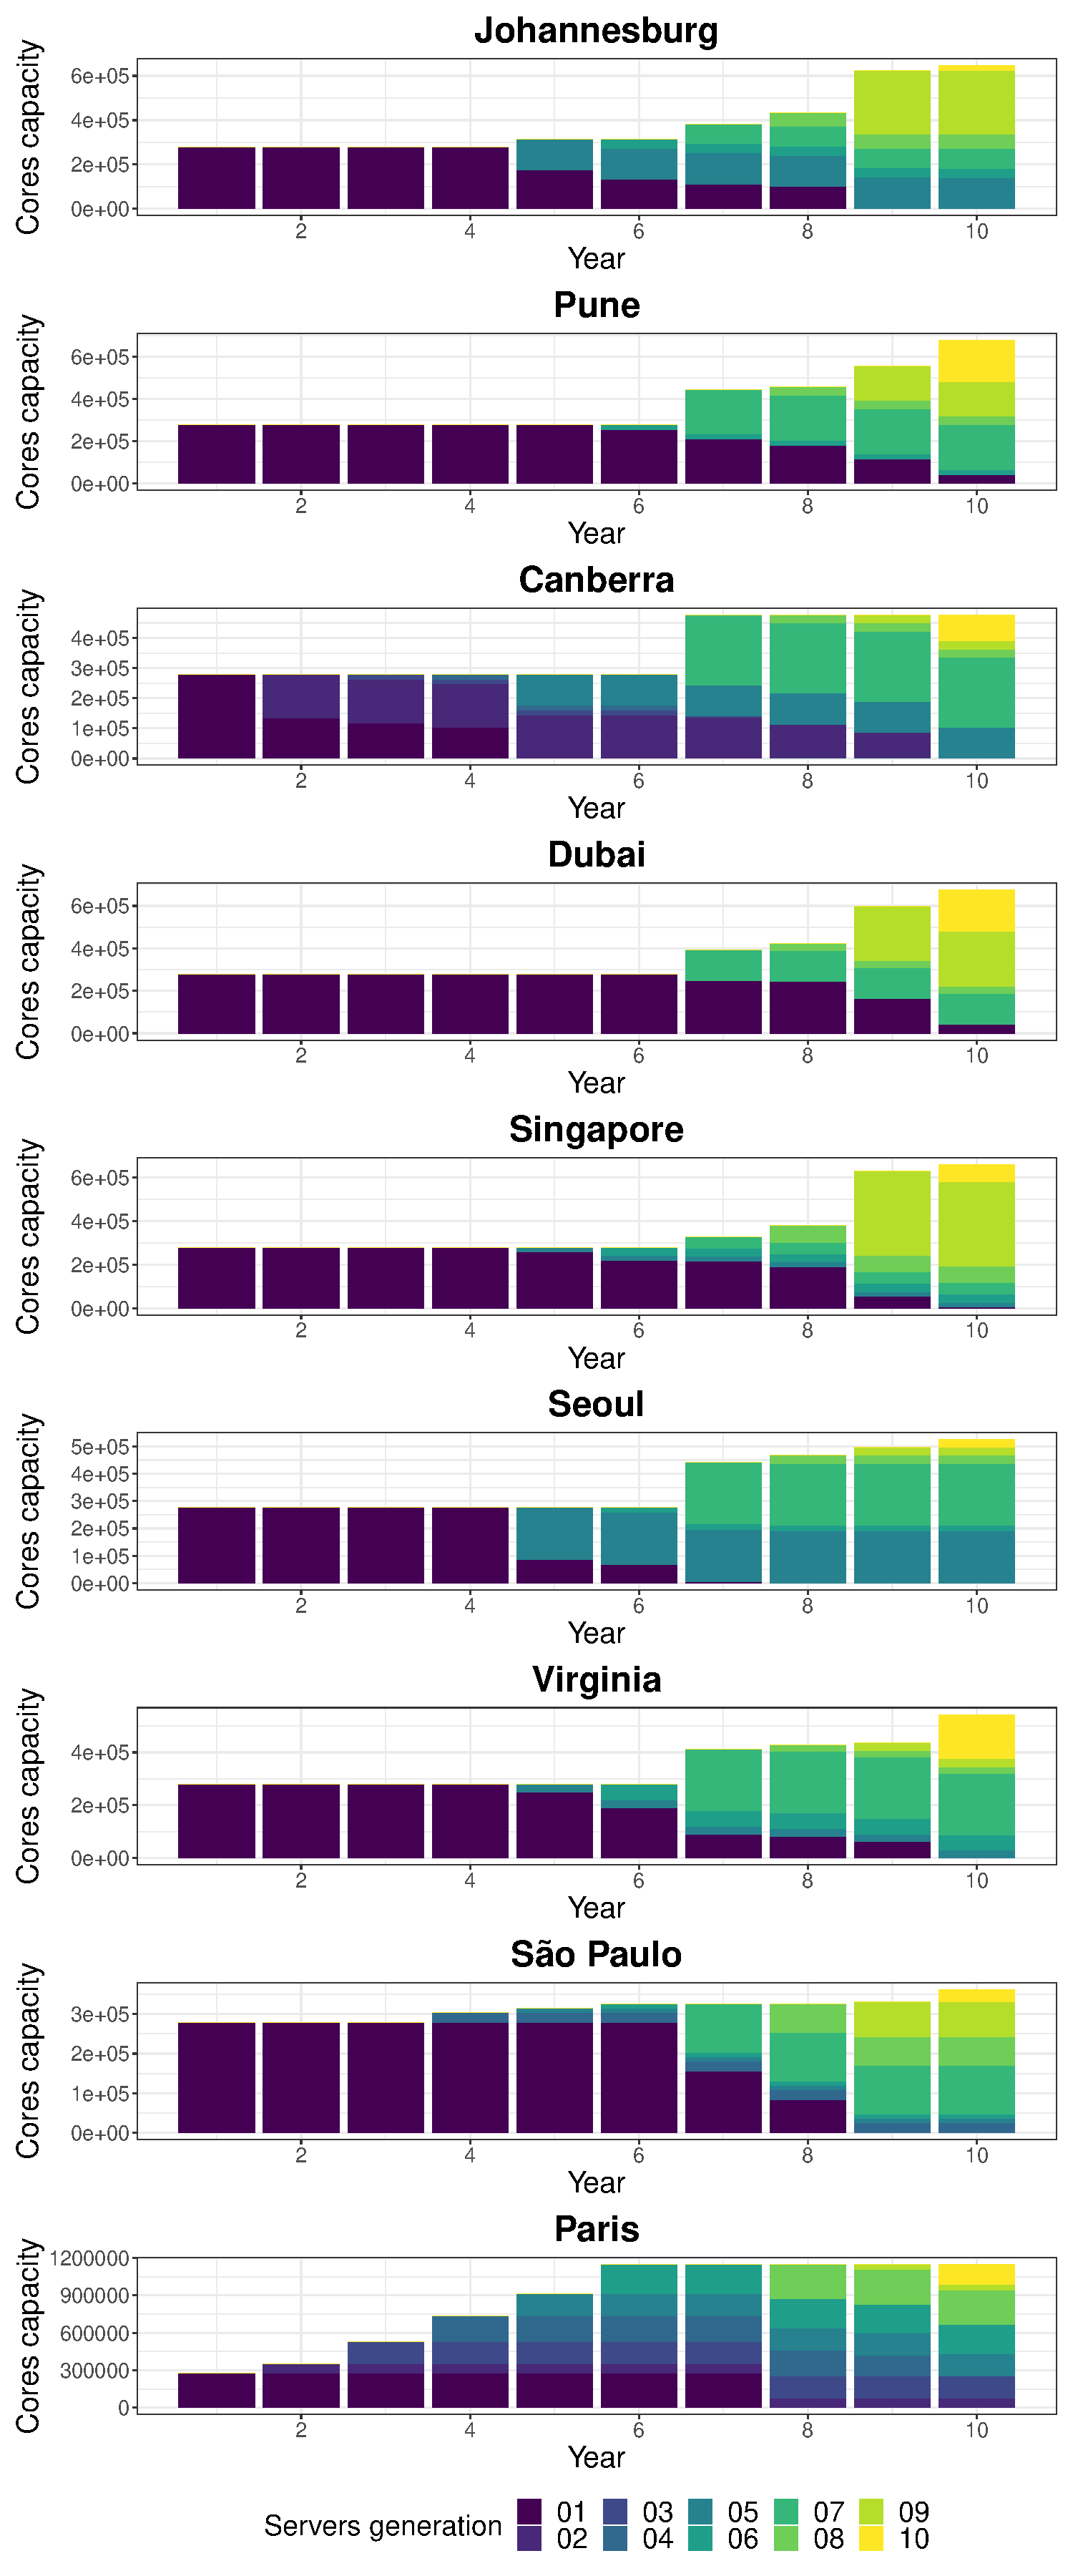
\includegraphics[width=\linewidth]{images/dc_evolution_year_by_year.pdf}
  \caption{Sizing with information of the current year.}
  \label{fig:dc_evolution_year_by_year}
\end{minipage}%
\begin{minipage}{.5\textwidth}
  \centering
  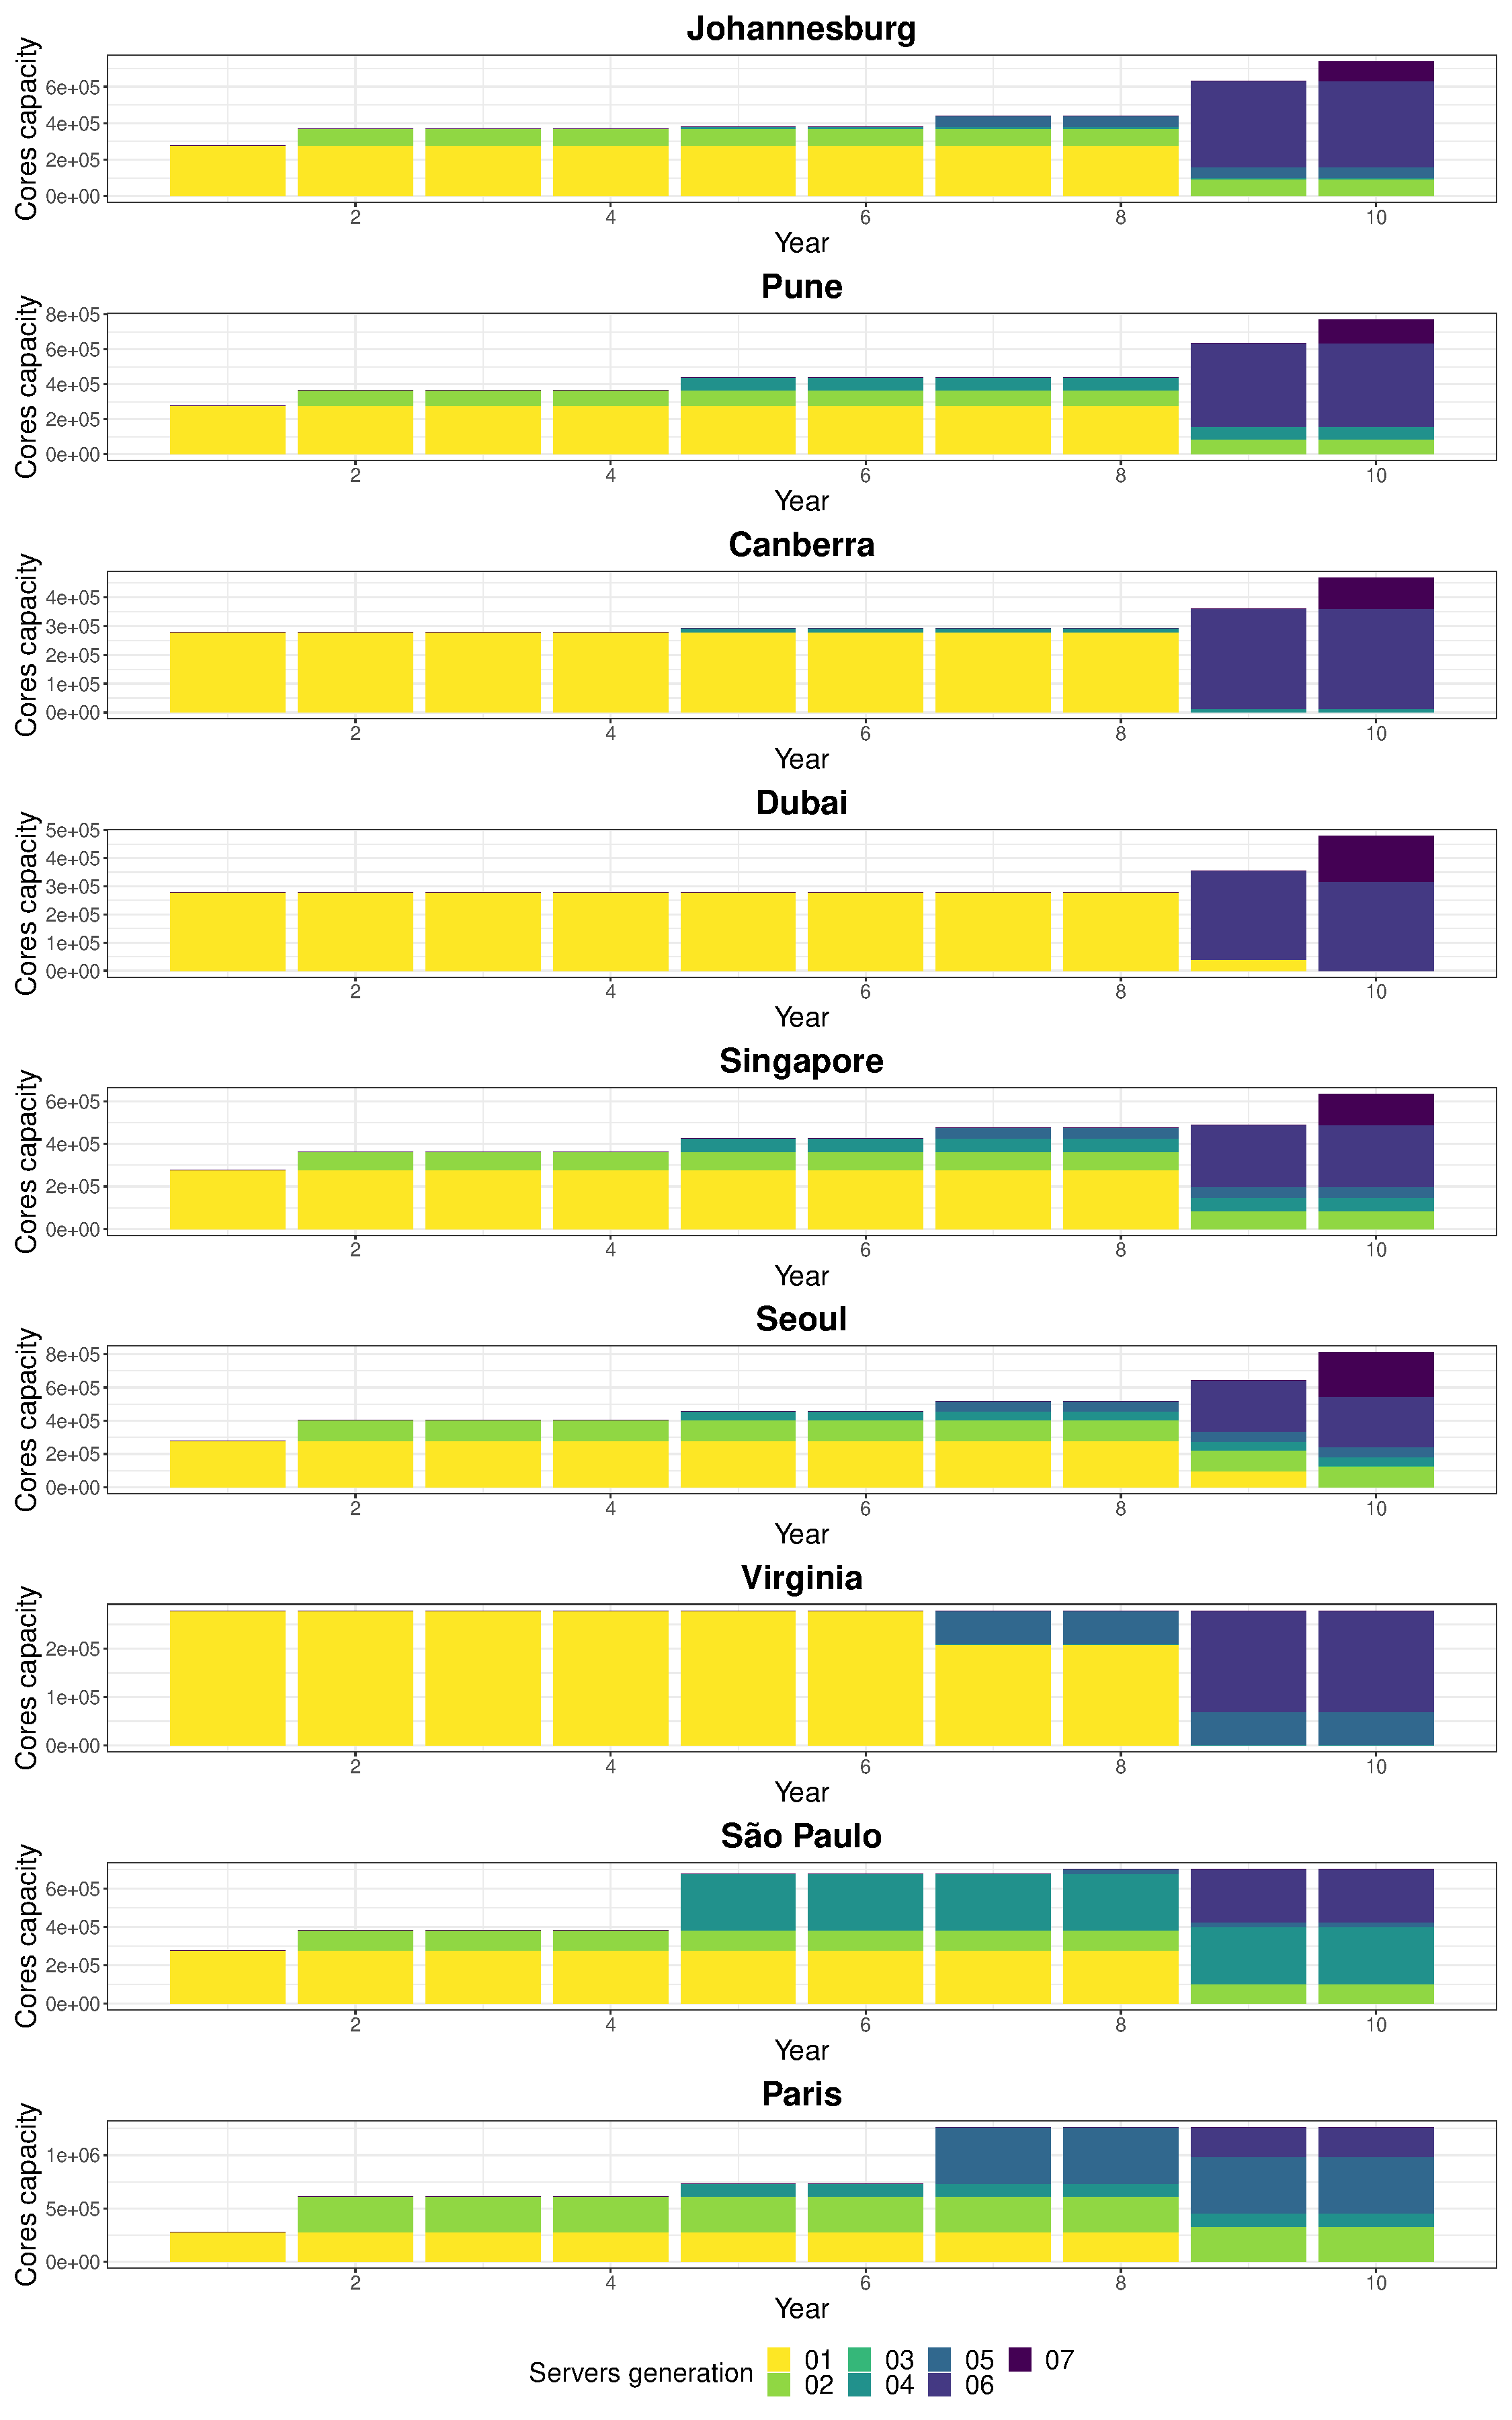
\includegraphics[width=\linewidth]{images/dc_evolution_optimal.pdf}
  \caption{Sizing knowing all information of the 10 years.}
  \label{fig:dc_evolution_optimal}
\end{minipage}
\end{figure}


\section{Discussion}


% talk about life cycle

% talk about sizing sensitivity

% talk about flexibility in the scheduling

We can extract two interesting information from the results. The first is that the reduction on the carbon emissions seems to have a limit (1.57\%). This can be justified by the fact that there are no much difference in the climate conditions during the interval of one week, or that the DC which would reduce the carbon emissions is already at peak capacity and cannot receive more workload. The second interesting observation is that by delaying a small portion of the workload (for example 10\% to 20\%)  the reduction is already really close to the maximum value. The reduction in the carbon emissions is low, but it is not negligible, since the order of magnitude of the emissions in a year of the cloud-federation is hundreds of tons of \ch{CO2} eq. Furthermore, it can compensate the impact of the climate conditions intermittency in the sizing, as we in a previous section that the result is up to 2\% far from the optimal.


% talk about price ...

% talk about new servers ...

\section{Summary}

\begin{itemize}

  \item Ongoing work:
    
  \item Studying the sensibility of the model to intermittency
    
    \begin{itemize}
      
    \item Simple methods are efficient (avg. or median of irradiation)

    \end{itemize}

  \item Other strategies to reduce the \ch{CO2} emissions

    \begin{itemize}
      
    \item Wind power: 6\% of reduction
    \item Delaying workload: up to 1.57\% of reduction
      
    \end{itemize}
    
  \item When to add/replace servers

    \begin{itemize}
      
    \item Year by year solution 8\% worse than the optimal

      
    \end{itemize}
    
    
  \end{itemize}
Future work:   Sizing for the long term :

  \begin{itemize}
    
  \item What could be learned from the optimal solution of adding/replacing servers ?
  \item Costs of the servers     
  \item Flexibility in the scheduling to reduce the number of
    servers manufactured
  \item Degradation of the renewable infrastructure over the years
    
  \end{itemize}    
